\hypertarget{introduction}{%
\section{Introduction}\label{introduction}}

Most research on AI for innovation asks about outcomes. Are LLM ideas as good as human ones \citep{Si2024, Terwiesch2026}? Do people generate better ideas with AI than without it \citep{Doshi2024, Anderson2024}? Does an agentic pipeline beat a single prompt, or a human team \citep{Liu2026, Massoudi2026}? These comparisons expire. Every model generation raises the outcome and lowers its price, so a finding that a model does or does not reach human level says more about the model of the day than about how to innovate with AI.

A question that lasts longer is how to \textbf{present the problem} to the model. The same task can be shown as a full structured model of the product, as the part of it that bears on the problem, or not at all. Whichever model is current, a team still has to decide what goes into the prompt and how much to pay for it. The measure that matters is therefore \textbf{outcome per token}: how efficiently a way of presenting the problem turns compute into useful ideas. Cost-aware evaluation is becoming standard for LLM reasoning and agents \citep{Chen2024d, Wang2024, Kapoor2025}, but not yet for design ideation.

The outcome itself needs care. Brainstorming is a search for the few excellent ideas among many, so what matters is the best ideas, not the average \citep{Dahan2001, Girotra2010}. We measure \textbf{yield}: top ideas (the top ∼12\% of all ideas) per 100k tokens. Counted against tokens spent, top ideas accumulate in a straight line, so representations can be compared by slope.

We study this with an established structured product description, the \emph{innovation matrix} (IM) of Leo Tchirsky \citep{Tchirsky}: a typed graph linking \textbf{market needs → functions → components → enabling technologies}, with constraints and actors attached. The microwave-oven IM used here has 123 nodes and 246 edges. More context is not free even when it fits: long inputs can lower LLM performance \citep{Liu2024, Levy2024}, and retrieving the relevant part can match the whole at a fraction of the cost \citep{Li2024}. One model applies one innovation operator (SUBSTITUTE) for 13 market needs, with the prompt fixed and only the representation varied:

\begin{itemize}
\tightlist
\item
  \textbf{A, full graph:} the whole IM;
\item
  \textbf{B, market-need slice:} the target market need's vertical slice;
\item
  \textbf{R, random slice:} a size-matched random selection of nodes, separating relevance from size;
\item
  \textbf{C, no graph:} the product and the market need only.
\end{itemize}

These are crossed with four levels of thinking effort, the other main way to spend tokens: 580 calls and 2,892 ideas, judged blind by a second model, as whole sets and idea by idea. We ask:

\begin{itemize}
\tightlist
\item
  \textbf{RQ1.} Which representation yields the most top ideas per token?
\item
  \textbf{RQ2.} Does the amount or the relevance of the graph matter?
\item
  \textbf{RQ3.} How does spending tokens on context compare with spending them on thinking effort?
\end{itemize}

An exploratory follow-up asks whether the answer depends on the persona the model adopts \citep{Lu2024}: innovation engineer, lateral thinker \citep{Bono1970} or patent-focused inventor.

\textbf{Findings in brief.} The market-need slice at medium effort yields 8.8 top ideas per 100k tokens, about three times the full graph at any effort (2.6--3.2), and beats it on 10 of 13 market needs. The full graph wins whole-set comparisons, mainly through specificity, but no more of its ideas reach the top, and at twice the cost per call it is less efficient than no graph at all (3.1 against 6.4 at high effort). Relevance, not size, drives the gain: the market-need slice out-yields the size-matched random slice in 99\% of bootstrap draws, and the random slice is the least efficient graph form. More thinking effort raises quality but not yield. No persona beat the plain engineer per token.

\textbf{Contributions.}

\begin{itemize}
\tightlist
\item
  A framing of AI-ideation research around representation efficiency, outcome per token, instead of outcome benchmarks against humans or against no AI.
\item
  Yield, top ideas per token, as a top-tail measure that does not saturate and leads to different conclusions from mean scores.
\item
  A controlled comparison of four representations of one product graph, crossed with thinking effort and, exploratorily, persona, with all prompts, calls and judgements released.
\end{itemize}

\section{Related work}
\label{related-work}

\subsection{From quality charts to product graphs}

Structured descriptions that link what customers want to what a product does and what it is made of are older than computing in design. Quality function deployment began in Japanese manufacturing in the late 1960s, was taken up by Toyota and its suppliers in the 1970s, and reached Western industry as the ``house of quality'' \citep{ed2024,Hauser1988,Chan2002}. Its matrices relate customer requirements to engineering characteristics, and then to parts and processes, so that every design decision can be traced to a market need. Related schemes followed, each making a different link explicit: morphological analysis lays out the alternatives for each function \citep{Zwicky1967,Ritchey2006,Ritchey2018}; the design structure matrix records the dependencies between components \citep{Steward1981,Browning2001,Eppinger2012}; function--behaviour--structure separates what a design is for from what it is \citep{Gero1990,Gero2004}; the functional basis standardises the vocabulary of functions and flows \citep{Stone2000,Hirtz2002}; and technology roadmaps link market needs to products and technologies over time \citep{Phaal2004}. The innovation matrix used here \citep{Tchirsky,berengueres2014} combines several of these links in one layered graph, from market needs through functions and components to technologies and scientific fields (it is distinct from the design-led innovation matrix of \citet{Kyffin2009}). All of these were made for people, typically a team in front of a wall chart, who read them selectively.

\subsection{LLMs that innovate with design methods}

Language models were first used as concept generators \citep{Zhu2022,Ma2023} and compared with people: their concepts are less diverse than crowdsourced ones \citep{Ma2025}, their research ideas are judged more novel but slightly less feasible than experts' \citep{Si2024}, and working with them raises individual creativity while narrowing collective diversity \citep{Doshi2024,Anderson2024,Ashkinaze2025,Wadinambiarachchi2024}. Recent systems give the model the structured methods above. An FBS ontology steers concept generation \citep{Chen2024a}; generated text and images enrich concepts \citep{Chen2024}; TRIZ is applied by single models and by agent teams \citep{Chen2024c,Jiang2025,Szczepanik2025}; morphological analysis is automated \citep{Chen2024b}; and agentic workflows chain whole design processes \citep{Ding2023,Massoudi2026}. iDesignGPT \citep{Liu2026} goes furthest: agent clusters run problem definition with QFD and Kano analysis, then functional decomposition, morphological analysis, SCAMPER and TRIZ, and produce a product design specification. Persona prompts are a related device, from role-play that raises the creativity of LLM discussions \citep{Lu2024} to agents that act out a design team \citep{Liu2025}, drawing on ideas about thinking styles in innovation \citep{Bono1970,Kelley2005}.

\subsection{What ``innovative'' is checked against}

These systems claim to innovate, but the claim usually rests on ratings: experts or a model score novelty and originality, or embedding distances measure how far the generated concepts spread from each other. iDesignGPT, for example, reports that it ``surpasses benchmark models in generating innovative, modular, and rational solutions'', on the basis of expert scores against GPT-4o baselines and semantic novelty metrics; patents are searched as an input to the workflow, but the generated concepts are not compared with prior art \citep{Liu2026}. This is typical. Novelty is judged relative to other generated ideas or to a rater's memory, seldom against what already exists, although patent-based measures of technological novelty are well established \citep{Fleming2001,Verhoeven2016,Uzzi2013} and patent-derived knowledge networks are available for design \citep{Sarica2020,Luo2021}. An idea a rater finds novel may be on the market already. Our own study shares this limitation: its judge rates novelty and patentability from knowledge, without a prior-art search, and several of its top-rated ideas, such as solid-state RF heating and RF thawing, already exist in industry, as the judge itself noted. A second gap is cost: none of these systems reports what its outputs cost, so a more elaborate pipeline cannot be weighed against a simpler one.

\subsection{Context and cost in LLMs}

More context is not free even when it fits in the window. Models use information in the middle of long inputs poorly \citep{Liu2024}, their reasoning degrades as inputs grow long well before the limit \citep{Levy2024}, and they struggle when relevant content must be inferred rather than matched \citep{Modarressi2025}; retrieval can reach results comparable to long context at a fraction of the cost \citep{Li2024}. Elsewhere, cost is becoming a first-class outcome: cascades and routers match strong models at lower cost \citep{Chen2024d,Ong2024,Ding2024}, reasoning strategies are compared at equal token budgets \citep{Wang2024,Han2025}, and agent benchmarks report accuracy together with cost \citep{Kapoor2025,Wang2025}. This work concerns tasks with right answers. Ideation has none, and its efficiency has rarely been measured.

\subsection{Measuring ideation}

Ideation is usually assessed by quantity, quality, novelty and variety \citep{Shah2003}, or by novelty and usefulness together \citep{Sarkar2011}. But a brainstorm is worth its best ideas, since the rest are discarded: idea-generation processes should be compared on the quality of the best idea, not the average \citep{Girotra2010}, and extreme-value models describe how the best of many concepts improves with the number tested \citep{Dahan2001}. Mean scores, the usual summary in LLM ideation studies, hide exactly this difference. We combine the tail and the cost in one measure, top ideas per token, and vary only how the product is presented, holding the model, the method and the prompt fixed.

\hypertarget{methods}{%
\section{Methods}\label{methods}}

The experiment holds the model, the task and the prompt fixed, and varies only how much of the product graph the prompt contains (the \emph{representation}) and how long the model may think (the \emph{effort}). It measures what each combination produces and what it costs.

\hypertarget{product-graph}{%
\subsection{Product graph}\label{product-graph}}

\textbf{The innovation matrix.} The innovation matrix (IM) of Leo Tchirsky \citep{Tchirsky}, as taught in design-thinking workshops \citep{berengueres2014}, describes a product as stacked layers: the \textbf{market needs} it serves, the \textbf{functions} that serve them, the \textbf{components} that perform the functions, the \textbf{technologies} that make the components possible, and the scientific \textbf{fields} behind those technologies (Figure \ref{fig:im_brownbook}). Reading upwards answers \emph{why} a part exists; reading downwards answers \emph{how} a market need is met. Innovation happens by changing a link: a new technology enables a different component, a component takes over another's function, or a function is found to serve a market need nobody had linked it to. In a workshop the matrix is drawn on a wall; here it is a typed graph that a model can read.

\begin{figure}[tbp]
\centering
\IfFileExists{figures/brown_book_innovation_matrix.png}{\includegraphics[width=0.8\textwidth]{figures/brown_book_innovation_matrix.png}}{\fbox{\parbox[c][5cm][c]{0.9\textwidth}{\centering\small missing: \texttt{\detokenize{figures/brown_book_innovation_matrix.png}}}}}
\caption{An innovation matrix as drawn in the workshop material \citep{berengueres2014}.}
\label{fig:im_brownbook}
\end{figure}

\textbf{The microwave matrix.} The product is a countertop microwave oven, the simplest mechanical model: a timer knob, a power knob, a door button and an interior lamp. The authors built its IM by hand in a single YAML file (\texttt{microwave\_base\_graph.yaml}), adding two cross-cutting types the workshop matrix keeps beside it, constraints and actors. It has 123 nodes and 246 directed, typed edges (Figure \ref{fig:im_microwave}; all nodes listed in Appendix A).

\begin{figure}[tbp]
\centering
\IfFileExists{figures/0_innovation_matrix_M8.pdf}{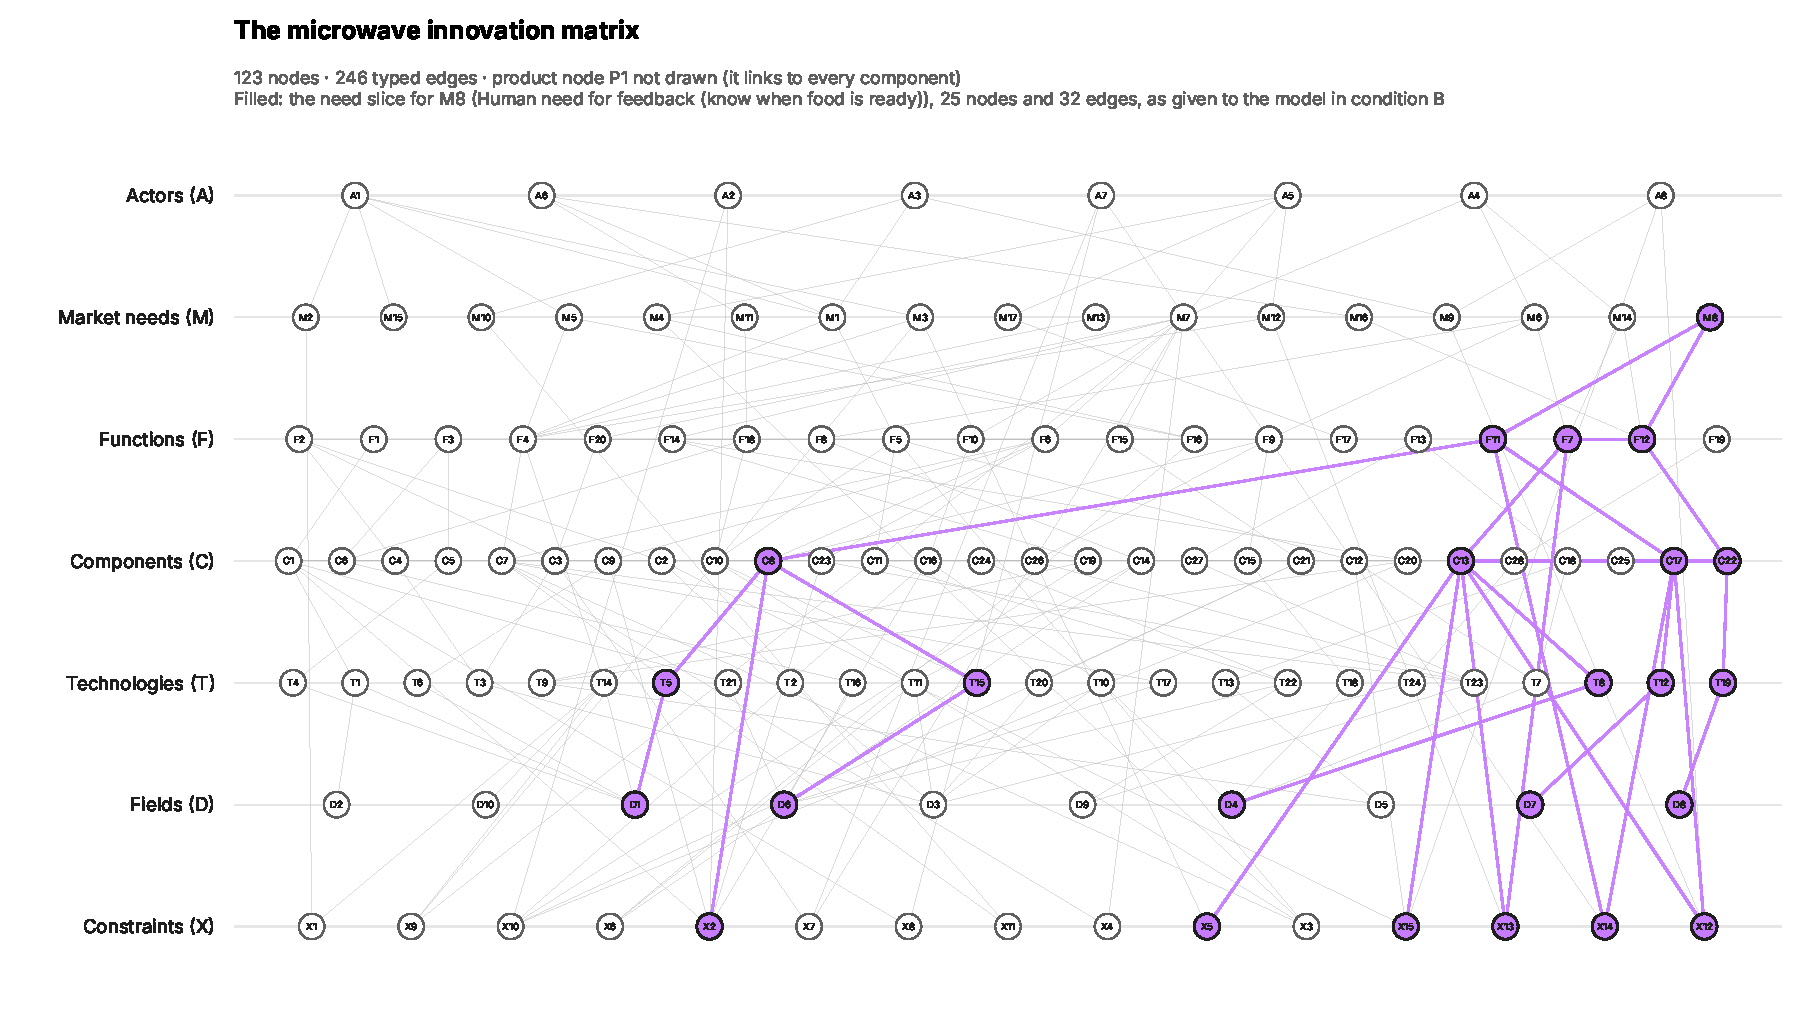
\includegraphics[width=\textwidth]{figures/0_innovation_matrix_M8.pdf}}{\fbox{\parbox[c][5cm][c]{0.9\textwidth}{\centering\small missing: \texttt{\detokenize{figures/0_innovation_matrix_M8.pdf}}}}}
\caption{The microwave innovation matrix used in the experiment. Rows are the layers, bottom to top, with constraints below and actors above. Filled nodes and edges are the market-need slice for M8, \emph{know when food is ready} (25 nodes, 32 edges): what the model sees in condition B for that market need, against the whole graph in condition A.}
\label{fig:im_microwave}
\end{figure}

\textbf{Nodes} belong to four stacked layers and four cross-cutting types:

\begin{longtable}[]{@{}
  >{\raggedright\arraybackslash}p{(\columnwidth - 4\tabcolsep) * \real{0.2258}}
  >{\raggedright\arraybackslash}p{(\columnwidth - 4\tabcolsep) * \real{0.0484}}
  >{\raggedright\arraybackslash}p{(\columnwidth - 4\tabcolsep) * \real{0.7258}}@{}}
\toprule\noalign{}
\begin{minipage}[b]{\linewidth}\raggedright
Type
\end{minipage} & \begin{minipage}[b]{\linewidth}\raggedright
Count
\end{minipage} & \begin{minipage}[b]{\linewidth}\raggedright
Role
\end{minipage} \\
\midrule\noalign{}
\endhead
\bottomrule\noalign{}
\endlastfoot
MarketNeed (M) & 17 & what users want (e.g.~M4 \emph{Defrost frozen food quickly}) \\
Function (F) & 20 & what the product does \\
Component (C) & 28 & physical parts \\
Technology (T) & 24 & the principles that enable components and functions \\
Field (D) & 10 & scientific fields the technologies are rooted in \\
Constraint (X) & 15 & limitations and conflicts (e.g.~X3 \emph{uneven heating}) \\
Actor (A) & 8 & user groups (e.g.~A5 \emph{parent with young children}) \\
Product (P) & 1 & the microwave oven \\
\end{longtable}

\textbf{Edges} carry one of twelve types. Those that build the layer stack are \texttt{has\_component}, \texttt{performs\_function}, \texttt{enables\_function}, \texttt{addresses\_need}, \texttt{enabled\_by} and \texttt{rooted\_in}. Component-level flows are \texttt{feeds} and \texttt{actuates}. Constraint links are \texttt{causes}, \texttt{contradicts} and \texttt{partially\_mitigates}. Weak associations are \texttt{relevant\_to}. A thirteenth type, \texttt{resolves}, is declared in the schema for agents to use when a new node replaces or solves an existing one; it does not occur in the base graph.

Each node has an identifier, type, label and a one-line detail. The file begins with a meta block that names the layers and defines the edge types.

\hypertarget{representations}{%
\subsection{Representations}\label{representations}}

Every prompt contains a graph file produced by one serializer from the base graph. Fields, ordering and the meta block are the same in every file; only \emph{which} nodes and edges are present differs. No file states which condition it belongs to. For each target market need \(M_k\) (\texttt{slicer.py}):

\begin{itemize}
\tightlist
\item
  \textbf{A, full graph.} All 123 nodes and 246 edges. One file shared by all market needs.
\item
  \textbf{B, market-need slice.} The vertical slice of \(M_k\), obtained by walking down the matrix from the market need:

  \begin{enumerate}
  \def\labelenumi{\arabic{enumi}.}
  \tightlist
  \item
    the functions that \texttt{addresses\_need} \(M_k\), plus every function that enables them through \texttt{enables\_function}, recursively;
  \item
    the components that \texttt{performs\_function} one of those functions;
  \item
    the technologies that enable those components or functions (\texttt{enabled\_by});
  \item
    the fields those technologies are \texttt{rooted\_in};
  \item
    every constraint linked to any node above by \texttt{causes}, \texttt{contradicts}, \texttt{partially\_mitigates} or \texttt{relevant\_to}, and every actor \texttt{relevant\_to} \(M_k\);
  \item
    the product node.
  \end{enumerate}

  The file contains the edges induced among the selected nodes.
\item
  \textbf{R, random slice.} The target market need and the product, plus a random draw of nodes with the same number of nodes of each type as B, with the induced edges. The draw is seeded by the market need identifier (\texttt{random.Random("\textless{}need\textgreater{}-1")}), so it is reproducible and independent of run order. R controls for the \emph{size} and layer composition of B while removing its \emph{relevance} to the market need.
\item
  \textbf{C, no graph.} The meta block (layer names and edge-type definitions) and the target market need node only.
\end{itemize}

Four needs (M2, M9, M10, M15) are not addressed by any function, so their vertical slice is empty. They were excluded, leaving 13 target market needs: M1, M3, M4, M5, M6, M7, M8, M11, M12, M13, M14, M16, M17.

\begin{longtable}[]{@{}
  >{\raggedright\arraybackslash}p{(\columnwidth - 8\tabcolsep) * \real{0.0625}}
  >{\raggedright\arraybackslash}p{(\columnwidth - 8\tabcolsep) * \real{0.4625}}
  >{\raggedright\arraybackslash}p{(\columnwidth - 8\tabcolsep) * \real{0.1000}}
  >{\raggedright\arraybackslash}p{(\columnwidth - 8\tabcolsep) * \real{0.0625}}
  >{\raggedright\arraybackslash}p{(\columnwidth - 8\tabcolsep) * \real{0.3125}}@{}}
\toprule\noalign{}
\begin{minipage}[b]{\linewidth}\raggedright
Condition
\end{minipage} & \begin{minipage}[b]{\linewidth}\raggedright
Nodes
\end{minipage} & \begin{minipage}[b]{\linewidth}\raggedright
Share of graph
\end{minipage} & \begin{minipage}[b]{\linewidth}\raggedright
Edges
\end{minipage} & \begin{minipage}[b]{\linewidth}\raggedright
Input tokens per call (mean, incl.~prompt)
\end{minipage} \\
\midrule\noalign{}
\endhead
\bottomrule\noalign{}
\endlastfoot
A & 123 & 100\% & 246 & 10,912 \\
B & 10--51 (median 45) & 8--42\% & 11--85 & 3,778 \\
R & 10--51, same as B for each market need & 8--42\% & 2--52 & 3,143 \\
C & 1 & 1\% & 0 & 1,055 \\
\end{longtable}

R matches B in node count and type composition but not in edges. Randomly drawn nodes are less connected to one another than the nodes of a vertical slice, so R contains fewer induced edges than B for every market need. It also uses 17\% fewer input tokens. R shares 3--29 nodes with B for the same market need, mostly by chance among the larger slices. A manifest (\texttt{slices/manifest.csv}) records, for every file, the node identifiers, counts per type, edge count, token count and SHA-256 hash.

\hypertarget{task-and-prompt}{%
\subsection{Task and prompt}\label{task-and-prompt}}

All calls use one prompt template (\texttt{template\_prompt.txt}, Appendix B). It asks the model to innovate the product ``based on the graph given'', encourages radical and wild ideas, and asks it to favour innovations that serve the target market need. Placeholders are filled by literal substitution: product name, target market need identifier and label, operator name and definition, the graph file, and the number of ideas.

\begin{itemize}
\tightlist
\item
  \textbf{Operator.} SCAMPER \emph{Substitute} in every call: ``Identify components and the functions they perform, then replace them with something cheaper or simpler that fulfils the same function equally well or better.''
\item
  \textbf{Worked example.} One example of an innovation the brief likes, taken from the authors' workshop material \citep{berengueres2014}. The door's mesh and the interior lamp both serve the user's need to see the food, so they can be replaced together by a webcam, or by a transparent casing that needs no lamp.
\item
  \textbf{Output.} Exactly 5 ideas as JSON. Each idea has a title; the identifiers of existing nodes it was applied to (\emph{anchors}); new nodes (type, label, one-line detail); new edges; and a one-sentence rationale for how it serves the target market need.
\end{itemize}

The prompt is identical across conditions except for the graph file. In condition C, the ``graph given'' is only the schema and the target market need.

\hypertarget{generation}{%
\subsection{Generation}\label{generation}}

\begin{itemize}
\tightlist
\item
  \textbf{Model.} \texttt{claude-haiku-5-5}, through the Anthropic Messages API, with streaming. No sampling parameters were set; the model does not accept a temperature setting, so all calls use its defaults.
\item
  \textbf{Thinking effort.} Set per call through the API's effort parameter, at four of the five available levels: low, medium (the model's default), high and xhigh. Thinking tokens are billed and reported as output tokens.
\item
  \textbf{Output limit.} 48,000 tokens (64,000 for xhigh). No call reached its limit.
\item
  \textbf{Design.} Five replicates per cell, each a fresh call with the identical prompt:
\end{itemize}

\begin{longtable}[]{@{}llll@{}}
\toprule\noalign{}
Conditions & Efforts & Needs & Calls \\
\midrule\noalign{}
\endhead
\bottomrule\noalign{}
\endlastfoot
A, B & low, medium, high & 13 & 390 \\
A, B & xhigh & 6 (M1, M4, M6, M8, M13, M17) & 60 \\
R, C & high & 13 & 130 \\
\textbf{Total} & & & \textbf{580} \\
\end{longtable}

The xhigh cells cover 6 market needs, chosen to span small and large slices, to limit cost. R and C were run at high effort only.

\begin{itemize}
\tightlist
\item
  \textbf{Parsing.} A response is valid if it parses as JSON with an \texttt{ideas} list. 579 of 580 calls were valid with 5 ideas; one returned no parseable ideas and is kept as a failure. In total, the calls produced 2,892 ideas.
\item
  \textbf{Logging.} The runner appends one JSON line per call to an append-only log (\texttt{runs/rq1\_full.jsonl}). Each line holds the run identifier (condition, market need, effort, replicate), the graph file's identifier and hash, the prompt hash, model, output limit, input and output tokens, latency, stop reason, the parsed ideas and the raw response. Runs are resumable, and cells can be added later without rerunning earlier ones.
\end{itemize}

\hypertarget{judging}{%
\subsection{Judging}\label{judging}}

Ideas were judged blind by a second, larger model, \texttt{claude-sonnet-5-5}, at medium effort, in two ways. In both, the judge saw each idea's \textbf{title, new elements (label and detail) and rationale only}. Node identifiers, anchors, edges, condition, effort and run identifiers were removed, so nothing revealed which graph the idea came from. The brief shown to the judge gave the product, target market need, operator, and the instruction that radical, wild ideas serving the market need were wanted.

\textbf{Pairwise set judging.} Two idea sets for the same market need and replicate, differing in one factor, were shown side by side. The judge scored each set from 1 to 5 on relevance, novelty, feasibility, specificity and diversity (how different the ideas are from each other), and named the better set or a tie (prompt in Appendix C). Every pair was judged twice, once in each presentation order, and the two verdicts were combined into one result per pair: agreeing verdicts count as a win, opposite verdicts as a tie. If one side had no parsed ideas, the other won without a judge call (one pair per affected comparison). The comparisons judged were:

\begin{longtable}[]{@{}lll@{}}
\toprule\noalign{}
Comparison & Effort & Pairs \\
\midrule\noalign{}
\endhead
\bottomrule\noalign{}
\endlastfoot
A vs B & low, high & 65 each \\
B vs R, B vs C, A vs C & high & 65 each \\
high vs low, within A and within B & --- & 65 each \\
xhigh vs high, within A and within B & --- & 30 each \\
B at high vs A at low & --- & 65 \\
\end{longtable}

\textbf{Individual idea scoring.} Each call's five ideas were sent to the judge in one request, with the instruction to rate each idea on its own merits, independently of the others. Each idea was scored from 1 to 5 on relevance, novelty, feasibility and specificity (prompts in Appendix D). An idea's \textbf{score} is the mean of the four ratings. All 2,892 ideas were scored; two calls whose first scoring returned the wrong number of ratings were scored again.

\hypertarget{measures}{%
\subsection{Measures}\label{measures}}

\textbf{Cost.} Input, output and total tokens per call, from the API's usage report.

\textbf{Use of the graph} (computed without model calls, from the parsed ideas):

\begin{itemize}
\tightlist
\item
  \emph{anchors outside the market-need slice}: the share of anchors that are existing nodes outside B's slice for that market need;
\item
  \emph{anchors not in the graph}: the share of anchors that match no node identifier in the base graph;
\item
  \emph{ideas echoing the worked example}: ideas whose title or new nodes mention a webcam, camera or transparency;
\item
  \emph{new nodes per idea}, and \emph{words per idea} in the text the judge sees.
\end{itemize}

\textbf{Top tail.} A \textbf{top idea} is one whose individual score is at least 4.0. Scores move in steps of 0.25 (one step of a 1--5 rating, averaged over four criteria), so no exact percentile cut exists; 4.0 is the step closest to the top 10\% and keeps 12.3\% of all ideas (355 of 2,892). As a stricter check, 4.25 keeps the top 2.4\% (68 ideas). Target market needs differ widely in how easily they yield top ideas (from 3\% to 29\% of ideas at 4.0), and the xhigh arms cover only 6 market needs, so every rate is computed per market need and then averaged over the market needs an arm was run on, each market need weighing the same. For each arm:

\begin{itemize}
\tightlist
\item
  \textbf{top-idea rate}: the market-need-averaged share of the arm's ideas that are top ideas;
\item
  \textbf{calls with a top idea}: the market-need-averaged share of calls producing at least one top idea;
\item
  \textbf{tokens per top idea}: the arm's total tokens divided by its number of top ideas;
\item
  \textbf{chance of a top idea for a budget} \(b\): the probability of at least one top idea when \(b\) tokens are spent on whole calls of that arm, averaged over market needs. For need \(j\), with \(p_j\) the share of calls containing a top idea and \(\bar t_j\) the mean tokens per call, \(k = \lfloor b / \bar t_j \rfloor\) calls succeed with probability \(1 - (1 - p_j)^k\). Calls are treated as independent. Because 5 calls per market need often give a raw share of exactly 0 or 1, \(p_j\) is the Jeffreys estimate \((h_j + \tfrac12)/(n_j + 1)\), where \(h_j\) of \(n_j\) calls contained a top idea.
\end{itemize}

\textbf{Mean idea score.} The market-need-averaged mean individual score per arm, and the mean of each criterion.

\hypertarget{statistics}{%
\subsection{Statistics}\label{statistics}}

\textbf{Pairwise judging.} The unit is the pair, not the verdict: the two presentation orders of a pair are not independent, so they are combined first. For each comparison:

\begin{itemize}
\tightlist
\item
  the \emph{win rate} of the first-named arm, with ties counting as half a win;
\item
  a Wilson 95\% confidence interval;
\item
  an exact two-sided sign test on wins against losses, ties excluded;
\item
  the \emph{order agreement}, the share of pairs that received the same verdict in both orders;
\item
  the mean score difference per criterion.
\end{itemize}

H2, that the market-need slice is no worse than the full graph, is tested as non-inferiority with a margin of 45\%: B is non-inferior if the lower bound of its win-rate interval against A is above 45\%.

To check whether judges favour longer sets, each pairwise record stores the number of words each side showed the judge. The share of decided pairs won by the longer set is reported next to each win rate.

\textbf{Top tail.} 95\% confidence intervals for the top-idea rate and the call rate come from 2,000 bootstrap resamples. Each resample redraws calls with replacement within each market need, which keeps the five ideas of a call together and the market-need-averaged weighting fixed.

No correction for multiple comparisons was applied. Per-market-need results rest on 5 calls or pairs each and are reported only as patterns.

\hypertarget{what-was-planned-and-what-was-not}{%
\subsection{What was planned and what was not}\label{what-was-planned-and-what-was-not}}

\begin{itemize}
\tightlist
\item
  \textbf{Planned before the full run.}

  \begin{itemize}
  \tightlist
  \item
    The four conditions, including R and C as controls.
  \item
    The A vs B comparison at low and high effort, with H1 (the full graph yields better sets) and H2 (B non-inferior to A at a 45\% margin).
  \item
    The effort comparison, high vs low.
  \item
    H3 (B better than R) and H4 (graph better than no graph), to be tested by pairwise judging.
  \end{itemize}
\item
  \textbf{Added after the pilot.}

  \begin{itemize}
  \tightlist
  \item
    Medium and xhigh effort.
  \item
    The B-high vs A-low comparison.
  \item
    Judging in both orders, the length check, and individual idea scoring, which was first used to rank ideas for inspection.
  \end{itemize}
\item
  \textbf{Exploratory, defined after seeing the results.}

  \begin{itemize}
  \tightlist
  \item
    The top-tail analysis: the 4.0 threshold, top-idea rate, tokens per top idea and chance for a budget.
  \item
    The market-need-averaged mean idea scores.
  \end{itemize}
\end{itemize}

The top-tail measures follow from the purpose of brainstorming (Section 1), but they were chosen after the pairwise results were known and are reported as exploratory. Their conclusions about relevance (B against R) are not confirmed by the planned pairwise test (Section 4).

\hypertarget{pilot}{%
\subsection{Pilot}\label{pilot}}

A pilot (2 market needs, M8 and M16; A and B; low, medium and high effort; 3 replicates; 36 calls) tested the pipeline. It led to five changes:

\begin{itemize}
\tightlist
\item
  the output limit was raised from 8,000 to 48,000 tokens, after half the high-effort calls used up their budget thinking and returned no ideas;
\item
  calls were switched to streaming;
\item
  effort was added to the run identifier so cells could be resumed;
\item
  every pair was judged in both orders;
\item
  the length check was added.
\end{itemize}

The pilot's 17-of-18 advantage for the full graph did not survive at full scale (Section 4).

\hypertarget{human-validation-in-progress}{%
\subsection{Human validation (in progress)}\label{human-validation-in-progress}}

To test whether the judge's individual scores, and in particular its top tier, agree with people, a stratified sample of 99 ideas is being rated by three raters with engineering or product background, working independently (\texttt{human\_check.py}).

\begin{itemize}
\tightlist
\item
  \textbf{Sample.} Ideas are drawn by judge score band: 29 at ≥ 4.25, 30 at 4.0, 25 at 3.5--3.75 and 15 at ≤ 3.25. Within each band, the draw rotates across conditions and allows at most 3 ideas per market need.
\item
  \textbf{Rating sheet.} Raters see the market need, title, new elements and rationale. Condition, effort, scores and node identifiers are removed. They rate the same four criteria and say whether they would pursue the idea.
\item
  \textbf{Analysis.} Agreement between raters (Krippendorff's α, interval) and between raters and judge (Spearman's ρ). Also the probability that an idea the judge scores ≥ 4.0 receives a higher human score than one it scores below 4.0.
\end{itemize}

\hypertarget{reproducibility}{%
\subsection{Reproducibility}\label{reproducibility}}

The repository contains the base graph, the slicer and its manifest, the prompt template, the generation runner, the analysis scripts (\texttt{analyze.py}, \texttt{top\_ideas.py}, \texttt{tail\_charts.py}, \texttt{charts.py}, \texttt{human\_check.py}), the complete call log with raw responses, all judge outputs, and the derived tables. Every number in Section 4 is regenerated by four commands: \texttt{python\ analyze.py\ stats}, \texttt{python\ analyze.py\ summary}, \texttt{python\ top\_ideas.py\ report} and \texttt{python\ tail\_charts.py}. Total generation used about 8.6 million tokens.

\hypertarget{results}{%
\section{Results}\label{results}}

\hypertarget{summary}{%
\subsection{Summary}\label{summary}}

The aim of brainstorming is the rare great idea, not a good average, so the main measure here is the \textbf{top tail}: how often an arm produces an idea in the top ∼12\% of all ideas, and what each such idea costs.

\begin{itemize}
\tightlist
\item
  \textbf{A relevant slice of the graph finds top ideas fastest per token.} Counted against tokens spent, top ideas accumulate in a straight line for every arm, so each arm has a yield: top ideas per 100k tokens. The market-need slice (B) at medium effort yields 8.8, about three times the full graph (A) at any effort (2.6--3.2). B's top-idea rate is also the highest at equal effort (15\% at medium and high, against 10\% for no graph and for a random slice of the same size).
\item
  \textbf{The full graph (A) writes the best idea \emph{sets} but does not find more top ideas.} Judged as whole sets, A beats B 64\% of the time and no graph 74\% of the time. But its top-idea rate is no higher than B's, and its yield is about 3 top ideas per 100k tokens at every effort, half or less of B's: its advantage is the specificity of an average set, not more standout ideas.
\item
  \textbf{A graph helps, clearly so when it is the full graph.} A beats C on whole sets (74\%, p \textless{} 0.001); B beats C less clearly (62\%, p = 0.053) but has a higher top-idea rate (14.7\% vs 10.2\%).
\item
  \textbf{Relevance vs size is only partly settled.} In the top tail, the market-need slice beats the size-matched random slice (top-idea rate 14.7\% vs 9.8\%; yield 5.9 vs 4.1 per 100k tokens; the slice's slope is higher in 99\% of paired bootstrap draws). Judged as whole sets, the two cannot be told apart (B over R 54\%, p = 0.55). What a relevant slice adds shows up in the best ideas, not in the average set.
\item
  \textbf{The efficiency gain holds market need by market need, and is largest for small slices.} The slice is more efficient than the full graph on 10 of 13 market needs (sign test p = 0.039), and no graph beats a random slice on 10 of 12. The slice's lead is 3--5× for market needs whose slice has 15--28 nodes, and 1--2× for those with 45--51 nodes (exploratory).
\item
  \textbf{Persona prompting did not raise efficiency (exploratory follow-up).} On three market needs, neither a lateral-thinker nor a patent-focused persona beat the plain innovation engineer per token (6.3 top ideas per 100k tokens; patent persona 5.5, lateral thinker 4.3, lower than the engineer's in \textgreater{} 99.9\% of bootstrap draws); the lateral thinker was the least efficient, especially without a graph. The market-need slice helped every persona; whether it helps some personas more than others could not be resolved.
\item
  \textbf{Thinking effort is the strongest lever on quality, but not on yield.} High beats low in about 93\% of set comparisons, and xhigh produces the highest top-idea rates of all (19--21\%). But each call costs proportionally more, so yield does not rise with effort: for the full graph it stays at about 3 per 100k tokens from low to xhigh, and for the slice it peaks at medium (8.8) and falls at high (5.9) and xhigh (3.1).
\item
  \textbf{No graph is surprisingly efficient.} Its calls are the cheapest, so despite a low top-idea rate its yield (6.4) beats the random slice (4.1) and the full graph (3.1), and is close to the slice at high effort (5.9).
\end{itemize}

\hypertarget{setup}{%
\subsection{Setup}\label{setup}}

\begin{longtable}[]{@{}
  >{\raggedright\arraybackslash}p{(\columnwidth - 2\tabcolsep) * \real{0.2857}}
  >{\raggedright\arraybackslash}p{(\columnwidth - 2\tabcolsep) * \real{0.7143}}@{}}
\toprule\noalign{}
\begin{minipage}[b]{\linewidth}\raggedright
Item
\end{minipage} & \begin{minipage}[b]{\linewidth}\raggedright
Value
\end{minipage} \\
\midrule\noalign{}
\endhead
\bottomrule\noalign{}
\endlastfoot
Product graph & \texttt{microwave\_base\_graph.yaml}: 123 nodes, 246 edges \\
Target needs & 13: M1, M3, M4, M5, M6, M7, M8, M11, M12, M13, M14, M16, M17 (M2, M9, M10, M15 excluded: no functions address them, so their slice is empty) \\
Conditions & \textbf{A} = full graph · \textbf{B} = vertical slice of the target market need (functions, components, technologies, fields, linked constraints and actors) · \textbf{R} = random slice with the same number of nodes per layer as B · \textbf{C} = no graph (product description and target market need only) \\
Thinking effort & A and B: low, medium, high on all 13 market needs, xhigh on 6 market needs (M1, M4, M6, M8, M13, M17) · R and C: high on all 13 market needs \\
Replicates & 5 per cell \\
Generation calls & 580: A and B 450 (13 market needs × 2 conditions × 3 efforts × 5 reps, plus 6 market needs × 2 × 5 at xhigh); R and C 130 (13 × 2 × 5) \\
Prompt & \texttt{template\_prompt.txt}: 5 radical ideas for the target market need, operator SUBSTITUTE, worked example (door holes + lamp → webcam / transparent casing), JSON output \\
\texttt{max\_tokens} & 48,000 (64,000 for xhigh); no call was truncated \\
Sampling & model defaults (Haiku 5.5 accepts no temperature setting) \\
Pairwise judging & A vs B at low and high effort; B vs R, B vs C, A vs C at high effort; effort steps within A and B; B-high vs A-low. Blind comparison of two idea sets for the same market need and replicate; no condition labels or node IDs shown; each pair judged in both presentation orders and the two verdicts combined (agreeing verdicts = a win, split = a tie); scores 1--5 on relevance, novelty, feasibility, specificity, diversity \\
Individual scoring & every idea scored on its own, blind, 1--5 on relevance, novelty, feasibility, specificity; idea score = mean of the four (all 2,892 ideas) \\
Statistics & pairwise: per pair (65 pairs per comparison, 30 for xhigh), ties count half, Wilson 95\% CI, exact sign test · tail: rates averaged over market needs (each market need weighs the same), 95\% CI by resampling calls within each market need (2,000 resamples) \\
\end{longtable}

\hypertarget{cost-and-validity}{%
\subsection{Cost and validity}\label{cost-and-validity}}

\begin{figure}[tbp]
\centering
\IfFileExists{figures/1_tokens_per_call.png}{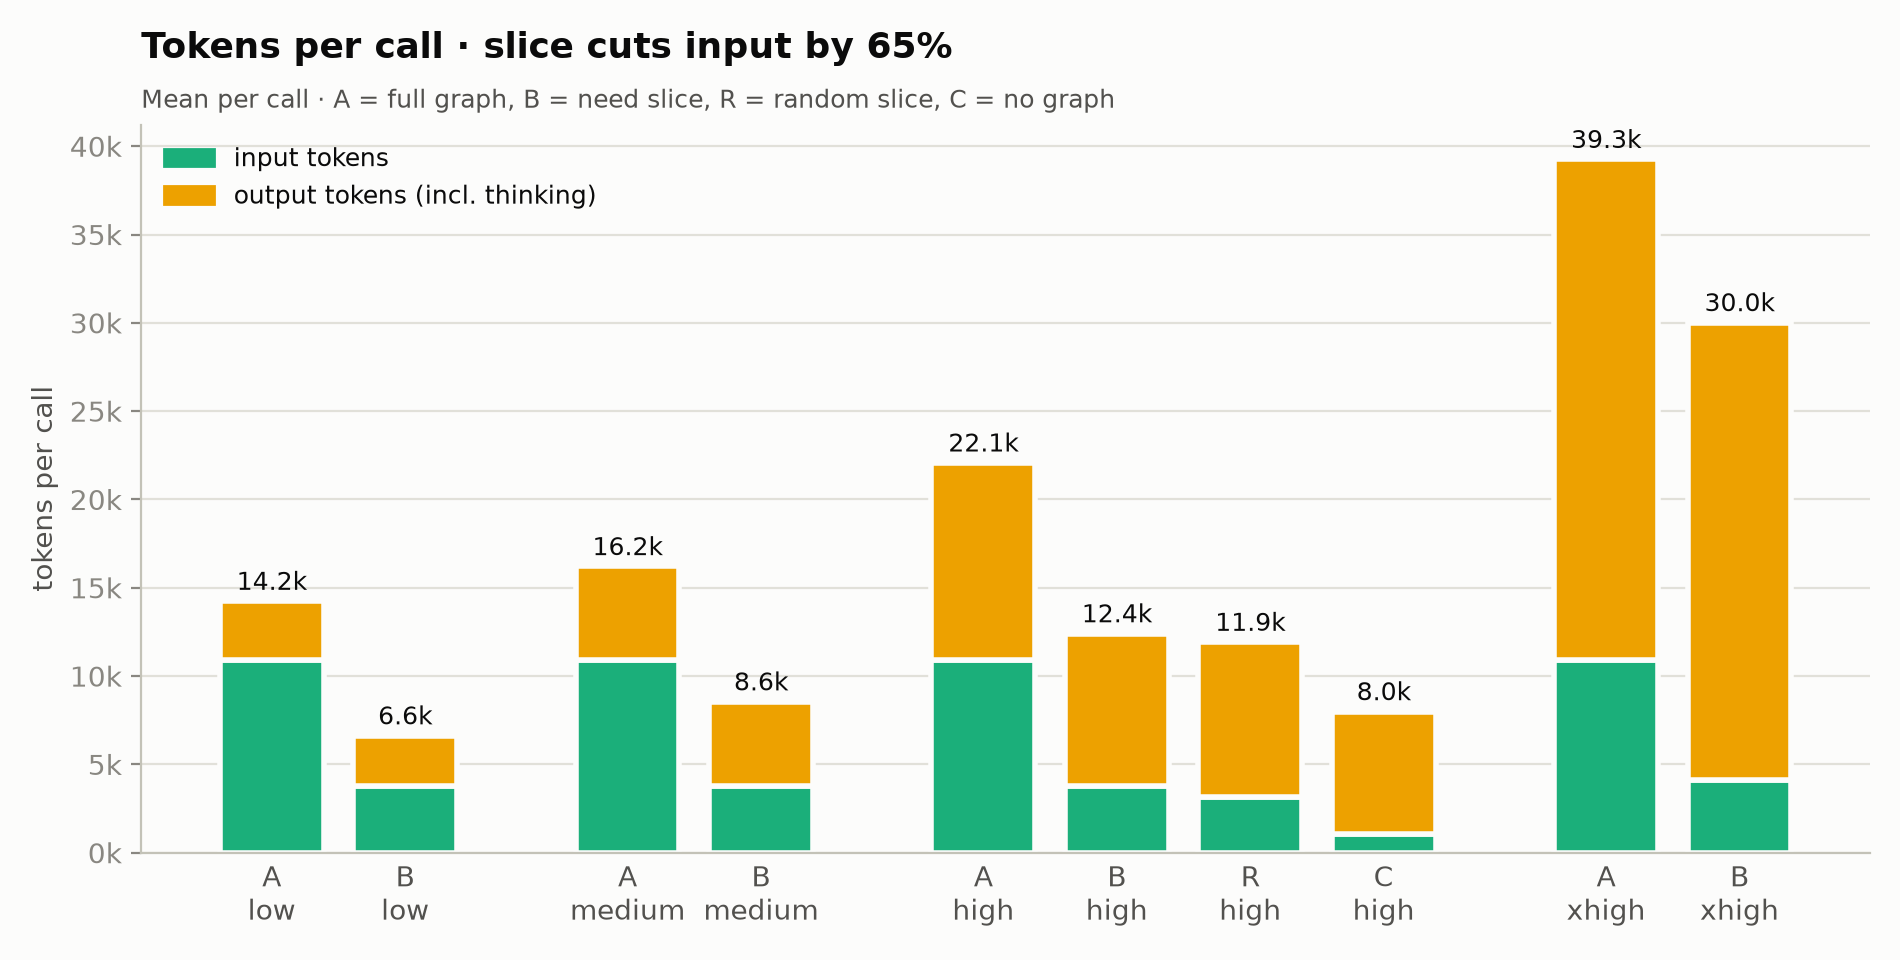
\includegraphics[width=\textwidth]{figures/1_tokens_per_call.png}}{\fbox{\parbox[c][5cm][c]{0.9\textwidth}{\centering\small missing: \texttt{\detokenize{figures/1_tokens_per_call.png}}}}}
\caption{Mean tokens per call by representation and effort, split into input (the prompt, most of it the graph file) and output (thinking and answer). The full graph pays for its context on every call; thinking effort drives the output for every representation.}
\label{fig:tokens}
\end{figure}

\begin{figure}[tbp]
\centering
\IfFileExists{figures/5_context_ladder.png}{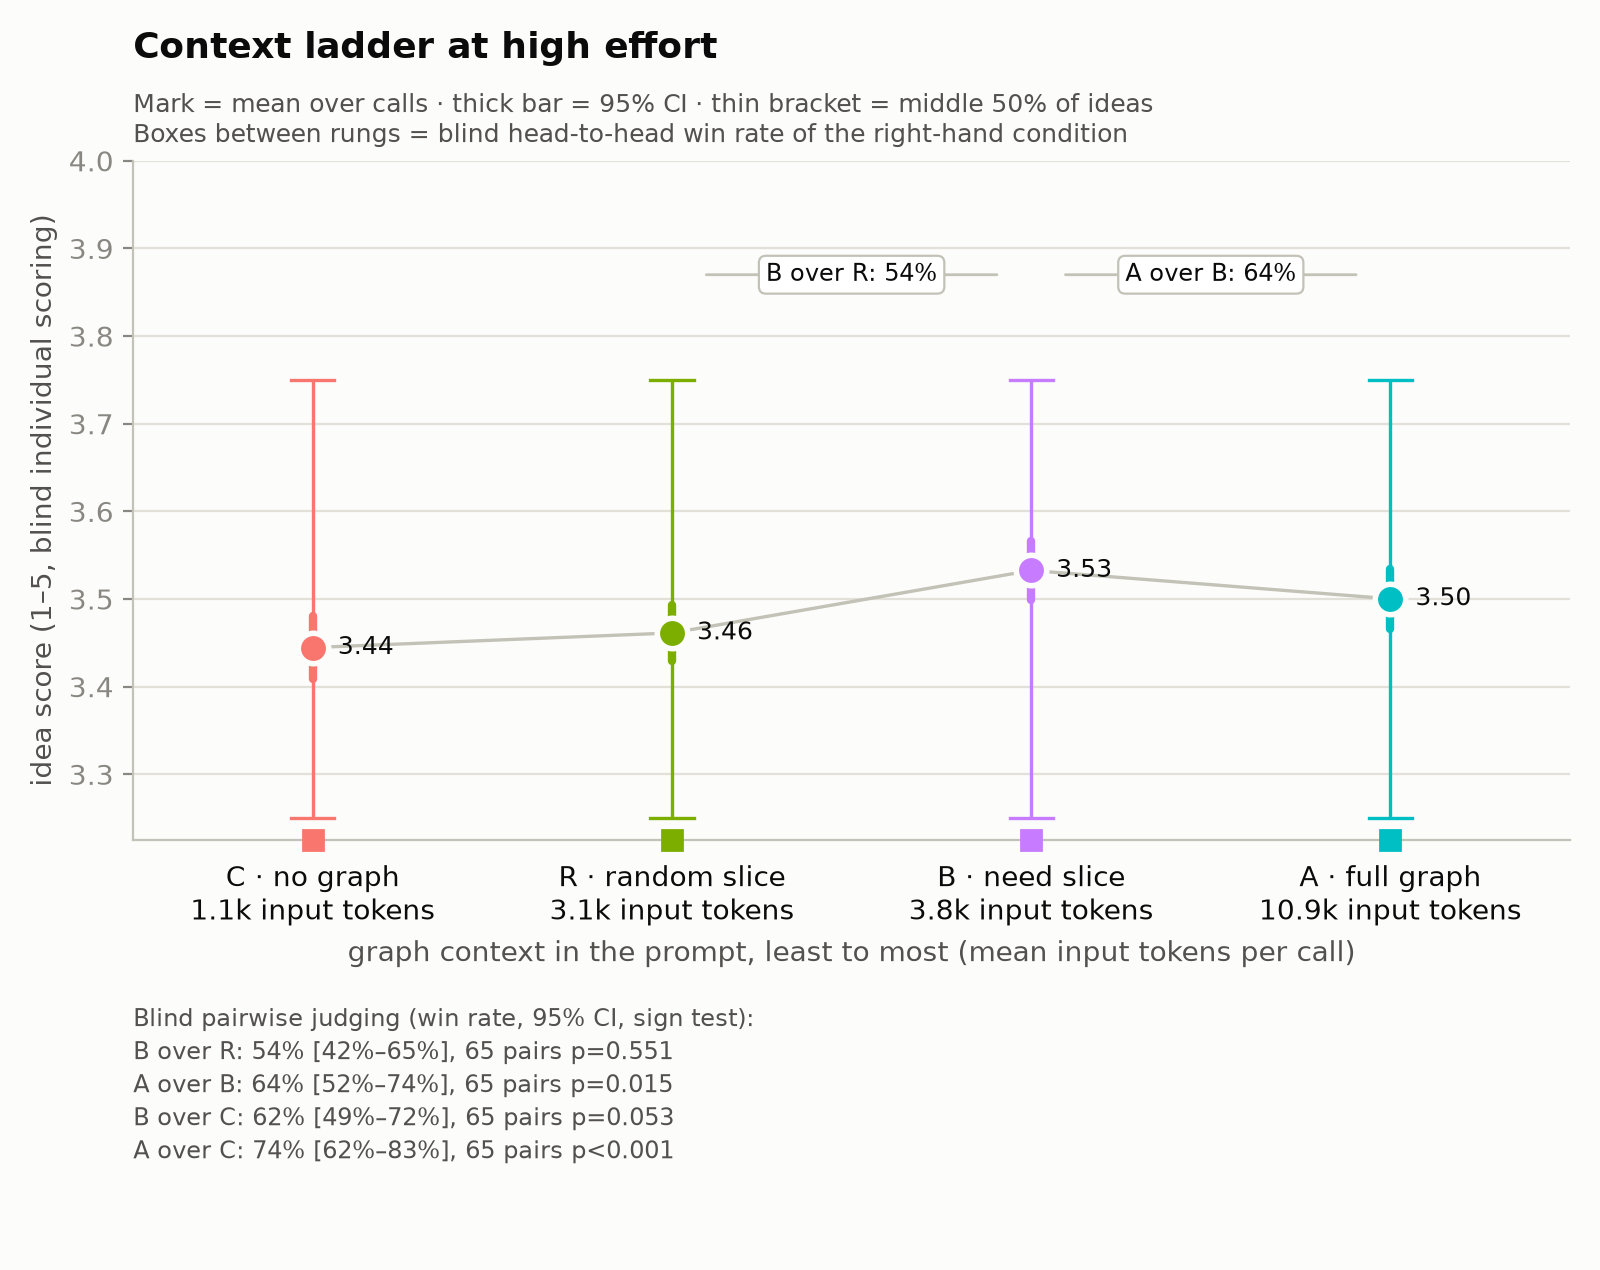
\includegraphics[width=\textwidth]{figures/5_context_ladder.png}}{\fbox{\parbox[c][5cm][c]{0.9\textwidth}{\centering\small missing: \texttt{\detokenize{figures/5_context_ladder.png}}}}}
\caption{The context ladder at high effort: no graph (C), random slice (R), market-need slice (B) and full graph (A), in order of input size, against mean idea score, with the head-to-head set win rates between rungs.}
\label{fig:ladder}
\end{figure}

Figure \ref{fig:tokens} shows tokens per call by condition and effort; Figure \ref{fig:ladder} sets the four representations side by side at high effort, input tokens against mean idea score.

Means per call.

\begin{longtable}[]{@{}
  >{\raggedright\arraybackslash}p{(\columnwidth - 14\tabcolsep) * \real{0.1020}}
  >{\raggedright\arraybackslash}p{(\columnwidth - 14\tabcolsep) * \real{0.1224}}
  >{\raggedright\arraybackslash}p{(\columnwidth - 14\tabcolsep) * \real{0.0612}}
  >{\raggedright\arraybackslash}p{(\columnwidth - 14\tabcolsep) * \real{0.1224}}
  >{\raggedright\arraybackslash}p{(\columnwidth - 14\tabcolsep) * \real{0.1429}}
  >{\raggedright\arraybackslash}p{(\columnwidth - 14\tabcolsep) * \real{0.1429}}
  >{\raggedright\arraybackslash}p{(\columnwidth - 14\tabcolsep) * \real{0.1429}}
  >{\raggedright\arraybackslash}p{(\columnwidth - 14\tabcolsep) * \real{0.1633}}@{}}
\toprule\noalign{}
\begin{minipage}[b]{\linewidth}\raggedright
Condition
\end{minipage} & \begin{minipage}[b]{\linewidth}\raggedright
Effort
\end{minipage} & \begin{minipage}[b]{\linewidth}\raggedright
Calls
\end{minipage} & \begin{minipage}[b]{\linewidth}\raggedright
Parse rate
\end{minipage} & \begin{minipage}[b]{\linewidth}\raggedright
Input tokens
\end{minipage} & \begin{minipage}[b]{\linewidth}\raggedright
Output tokens
\end{minipage} & \begin{minipage}[b]{\linewidth}\raggedright
Total tokens
\end{minipage} & \begin{minipage}[b]{\linewidth}\raggedright
Words per idea
\end{minipage} \\
\midrule\noalign{}
\endhead
\bottomrule\noalign{}
\endlastfoot
A & low & 65 & 100\% & 10,912 & 3,331 & 14,243 & 91 \\
A & medium & 65 & 100\% & 10,912 & 5,295 & 16,208 & 99 \\
A & high & 65 & 100\% & 10,912 & 11,163 & 22,076 & 108 \\
A & xhigh & 30 & 100\% & 10,912 & 28,346 & 39,258 & 117 \\
B & low & 65 & 100\% & 3,778 & 2,849 & 6,627 & 89 \\
B & medium & 65 & 100\% & 3,778 & 4,772 & 8,550 & 98 \\
B & high & 65 & 98.5\% & 3,778 & 8,628 & 12,407 & 100 \\
B & xhigh & 30 & 100\% & 4,135 & 25,885 & 30,020 & 117 \\
R & high & 65 & 100\% & 3,143 & 8,778 & 11,921 & 98 \\
C & high & 65 & 100\% & 1,055 & 6,939 & 7,994 & 106 \\
\end{longtable}

xhigh was run on 6 of the 13 market needs; those market needs have larger slices on average, which is why B's xhigh input is higher.

\begin{itemize}
\tightlist
\item
  \textbf{Input:} the slice cuts input tokens by 65\% on average (slices range from 10 to 51 nodes, 8--42\% of the graph). R matches B's node counts per layer but uses 17\% fewer input tokens, because random nodes have shorter labels and fewer linking edges; the size match is close but not exact.
\item
  \textbf{Total:} the slice saves 53\% of total tokens at low effort, 47\% at medium, 44\% at high and 24\% at xhigh. Output grows steeply with effort and soon dominates the bill, so the input saving matters less and less.
\item
  \textbf{Output grows with context:} at high effort, output is 6.9k tokens with no graph, 8.6--8.8k with a slice (B or R) and 11.2k with the full graph. More context makes the model think and write more, a cost beyond the prompt itself.
\item
  \textbf{Output by effort:} each step up costs more than the last: +1,900--2,000 tokens from low to medium, +3,900--5,900 from medium to high, about +17,000 from high to xhigh.
\item
  \textbf{Validity:} 579 of 580 calls returned valid JSON with 5 ideas; none hit the token limit.
\end{itemize}

\hypertarget{how-the-ideas-use-the-graph}{%
\subsection{How the ideas use the graph}\label{how-the-ideas-use-the-graph}}

\begin{longtable}[]{@{}
  >{\raggedright\arraybackslash}p{(\columnwidth - 10\tabcolsep) * \real{0.0562}}
  >{\raggedright\arraybackslash}p{(\columnwidth - 10\tabcolsep) * \real{0.0674}}
  >{\raggedright\arraybackslash}p{(\columnwidth - 10\tabcolsep) * \real{0.2809}}
  >{\raggedright\arraybackslash}p{(\columnwidth - 10\tabcolsep) * \real{0.2135}}
  >{\raggedright\arraybackslash}p{(\columnwidth - 10\tabcolsep) * \real{0.2697}}
  >{\raggedright\arraybackslash}p{(\columnwidth - 10\tabcolsep) * \real{0.1124}}@{}}
\toprule\noalign{}
\begin{minipage}[b]{\linewidth}\raggedright
Condition
\end{minipage} & \begin{minipage}[b]{\linewidth}\raggedright
Effort
\end{minipage} & \begin{minipage}[b]{\linewidth}\raggedright
Anchors outside the market need's own slice
\end{minipage} & \begin{minipage}[b]{\linewidth}\raggedright
Anchors to nodes not in the graph
\end{minipage} & \begin{minipage}[b]{\linewidth}\raggedright
Ideas repeating the worked example (of 5)
\end{minipage} & \begin{minipage}[b]{\linewidth}\raggedright
New nodes per idea
\end{minipage} \\
\midrule\noalign{}
\endhead
\bottomrule\noalign{}
\endlastfoot
A & low & 53\% & 0\% & 0.95 & 2.8 \\
A & medium & 49\% & 0\% & 0.69 & 3.1 \\
A & high & 48\% & 0\% & 0.54 & 3.4 \\
A & xhigh & 40\% & 0\% & 0.33 & 3.6 \\
B & low & 0\% & 0\% & 0.86 & 2.9 \\
B & medium & 0\% & 0\% & 0.48 & 3.1 \\
B & high & 0\% & 0\% & 0.55 & 3.3 \\
B & xhigh & 0\% & 0\% & 0.40 & 3.9 \\
R & high & 42\% & 0\% & 0.51 & 3.3 \\
C & high & --- & 48\% & 0.37 & 4.4 \\
\end{longtable}

\begin{itemize}
\tightlist
\item
  With the full graph, about half of all anchors lie outside the target market need's slice: A uses its extra context to reach across the product.
\item
  With a random slice, 42\% of anchors fall outside the market need's slice, because most of what R shows is unrelated to the market need.
\item
  With no graph, the model invents node IDs for half of its anchors and adds more new nodes per idea (4.4): it builds its own picture of the product instead of working on the given one.
\item
  Repetition of the worked example falls with effort, and is lowest with no graph.
\end{itemize}

\hypertarget{the-top-tail-which-arm-finds-the-great-ideas}{%
\subsection{The top tail: which arm finds the great ideas?}\label{the-top-tail-which-arm-finds-the-great-ideas}}

A \textbf{top idea} scores ≥ 4.0 on the individual blind scoring. Scores move in 0.25 steps, so an exact top 10\% does not exist: ≥ 4.0 keeps the top 12.3\% of all ideas (355 of 2,892), ≥ 4.25 the top 2.4\% (68). Market market needs differ a lot in how easy a top idea is (29\% of M14's ideas reach 4.0, 3\% of M11's), so every rate is the mean of per-market-need rates.

\hypertarget{top-idea-rate-score-4.0}{%
\subsubsection{Top-idea rate (score ≥ 4.0)}\label{top-idea-rate-score-4.0}}

\begin{figure}[tbp]
\centering
\IfFileExists{figures/6_top_idea_rate.png}{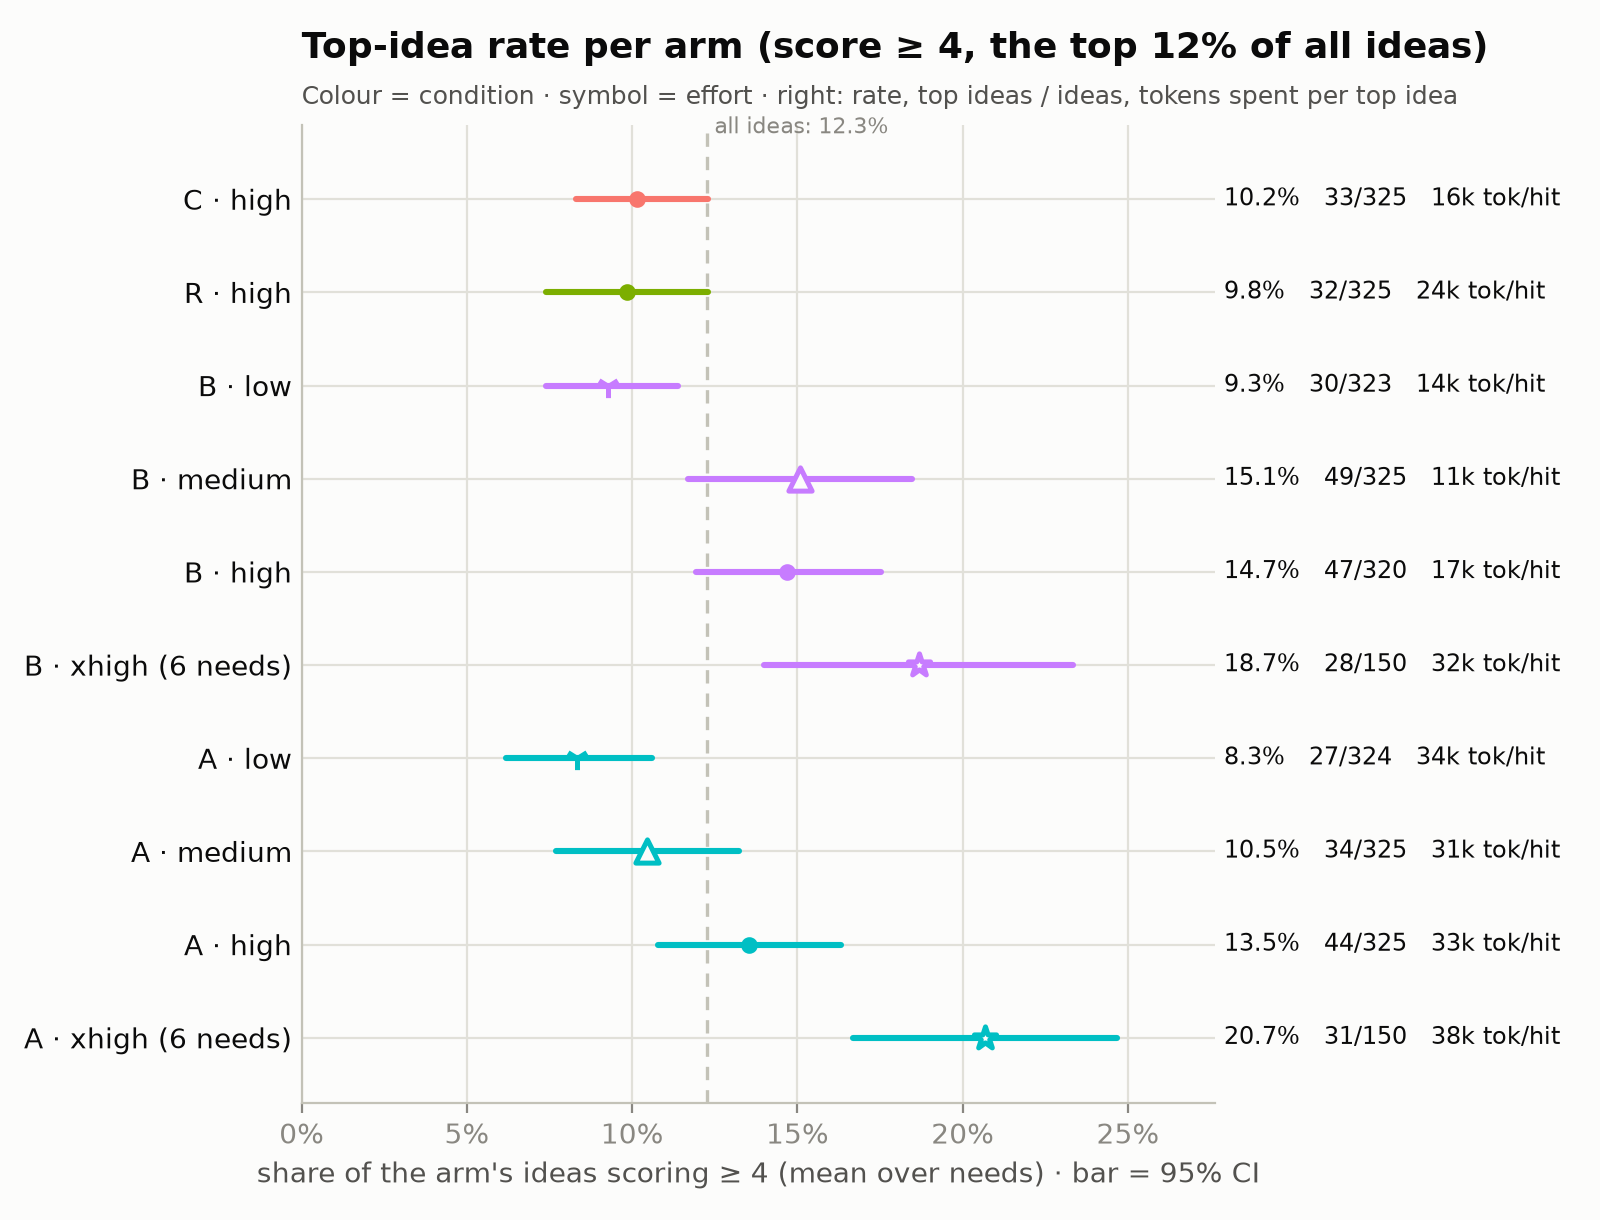
\includegraphics[width=\textwidth]{figures/6_top_idea_rate.png}}{\fbox{\parbox[c][5cm][c]{0.9\textwidth}{\centering\small missing: \texttt{\detokenize{figures/6_top_idea_rate.png}}}}}
\caption{Share of each arm's ideas that are top ideas (score $\geq$ 4.0, the top 12\% of all ideas), averaged over market needs, with 95\% intervals from resampling calls within market need. This is quality only; cost per call is not taken into account here.}
\label{fig:toprate}
\end{figure}

Figure \ref{fig:toprate} shows the rates with their intervals.

\begin{longtable}[]{@{}
  >{\raggedright\arraybackslash}p{(\columnwidth - 14\tabcolsep) * \real{0.1370}}
  >{\raggedright\arraybackslash}p{(\columnwidth - 14\tabcolsep) * \real{0.0411}}
  >{\raggedright\arraybackslash}p{(\columnwidth - 14\tabcolsep) * \real{0.1370}}
  >{\raggedright\arraybackslash}p{(\columnwidth - 14\tabcolsep) * \real{0.0959}}
  >{\raggedright\arraybackslash}p{(\columnwidth - 14\tabcolsep) * \real{0.1370}}
  >{\raggedright\arraybackslash}p{(\columnwidth - 14\tabcolsep) * \real{0.1781}}
  >{\raggedright\arraybackslash}p{(\columnwidth - 14\tabcolsep) * \real{0.1233}}
  >{\raggedright\arraybackslash}p{(\columnwidth - 14\tabcolsep) * \real{0.1507}}@{}}
\toprule\noalign{}
\begin{minipage}[b]{\linewidth}\raggedright
Arm
\end{minipage} & \begin{minipage}[b]{\linewidth}\raggedright
Needs
\end{minipage} & \begin{minipage}[b]{\linewidth}\raggedright
Top ideas / ideas
\end{minipage} & \begin{minipage}[b]{\linewidth}\raggedright
Top-idea rate
\end{minipage} & \begin{minipage}[b]{\linewidth}\raggedright
95\% CI
\end{minipage} & \begin{minipage}[b]{\linewidth}\raggedright
Calls with ≥ 1 top idea
\end{minipage} & \begin{minipage}[b]{\linewidth}\raggedright
Tokens per call
\end{minipage} & \begin{minipage}[b]{\linewidth}\raggedright
Tokens per top idea
\end{minipage} \\
\midrule\noalign{}
\endhead
\bottomrule\noalign{}
\endlastfoot
C · high & 13 & 33 / 325 & 10.2\% & 8.3--12.3\% & 48\% & 7,994 & 15,746 \\
R · high & 13 & 32 / 325 & 9.8\% & 7.7--12.3\% & 45\% & 11,921 & 24,215 \\
B · low & 13 & 30 / 323 & 9.3\% & 7.4--11.4\% & 37\% & 6,627 & 14,359 \\
B · medium & 13 & 49 / 325 & 15.1\% & 11.7--18.5\% & 52\% & 8,550 & \textbf{11,342} \\
B · high & 13 & 47 / 320 & 14.7\% & 11.9--17.5\% & 56\% & 12,384 & 16,838 \\
B · xhigh & 6 & 28 / 150 & 18.7\% & 14.0--23.3\% & 73\% & 30,020 & 32,164 \\
A · low & 13 & 27 / 324 & 8.3\% & 6.2--10.5\% & 37\% & 14,243 & 34,289 \\
A · medium & 13 & 34 / 325 & 10.5\% & 8.0--13.2\% & 45\% & 16,208 & 30,985 \\
A · high & 13 & 44 / 325 & 13.5\% & 10.5--16.3\% & 57\% & 22,076 & 32,612 \\
A · xhigh & 6 & 31 / 150 & 20.7\% & 16.7--24.7\% & 80\% & 39,258 & 37,991 \\
\end{longtable}

\begin{itemize}
\tightlist
\item
  \textbf{Relevance vs size (H3):} at the same effort and nearly the same size, the market-need slice yields top ideas at 14.7\% against 9.8\% for the random slice; the confidence intervals just touch. The whole-set judging does not confirm this (see below).
\item
  \textbf{Graph vs none (H4):} a relevant slice yields more top ideas than no graph (14.7\% vs 10.2\%); a random slice does not (9.8\%). The full graph is in between (13.5\%).
\item
  \textbf{Full graph vs slice:} at every effort, B's top-idea rate is equal to or higher than A's, at about half the tokens per top idea.
\item
  \textbf{Effort:} top-idea rates rise with effort for both A and B, with the largest rates at xhigh. But xhigh costs 2--3× the tokens per top idea of medium or high.
\item
  \textbf{Cheapest top ideas:} B at medium effort (11k tokens each), then B at low (14k), C (16k) and B at high (17k). A costs 31--38k at every effort.
\end{itemize}

\hypertarget{yield-top-ideas-per-100k-tokens}{%
\subsubsection{Yield: top ideas per 100k tokens}\label{yield-top-ideas-per-100k-tokens}}

\begin{figure}[tbp]
\centering
\IfFileExists{figures/8_top_ideas_vs_tokens.png}{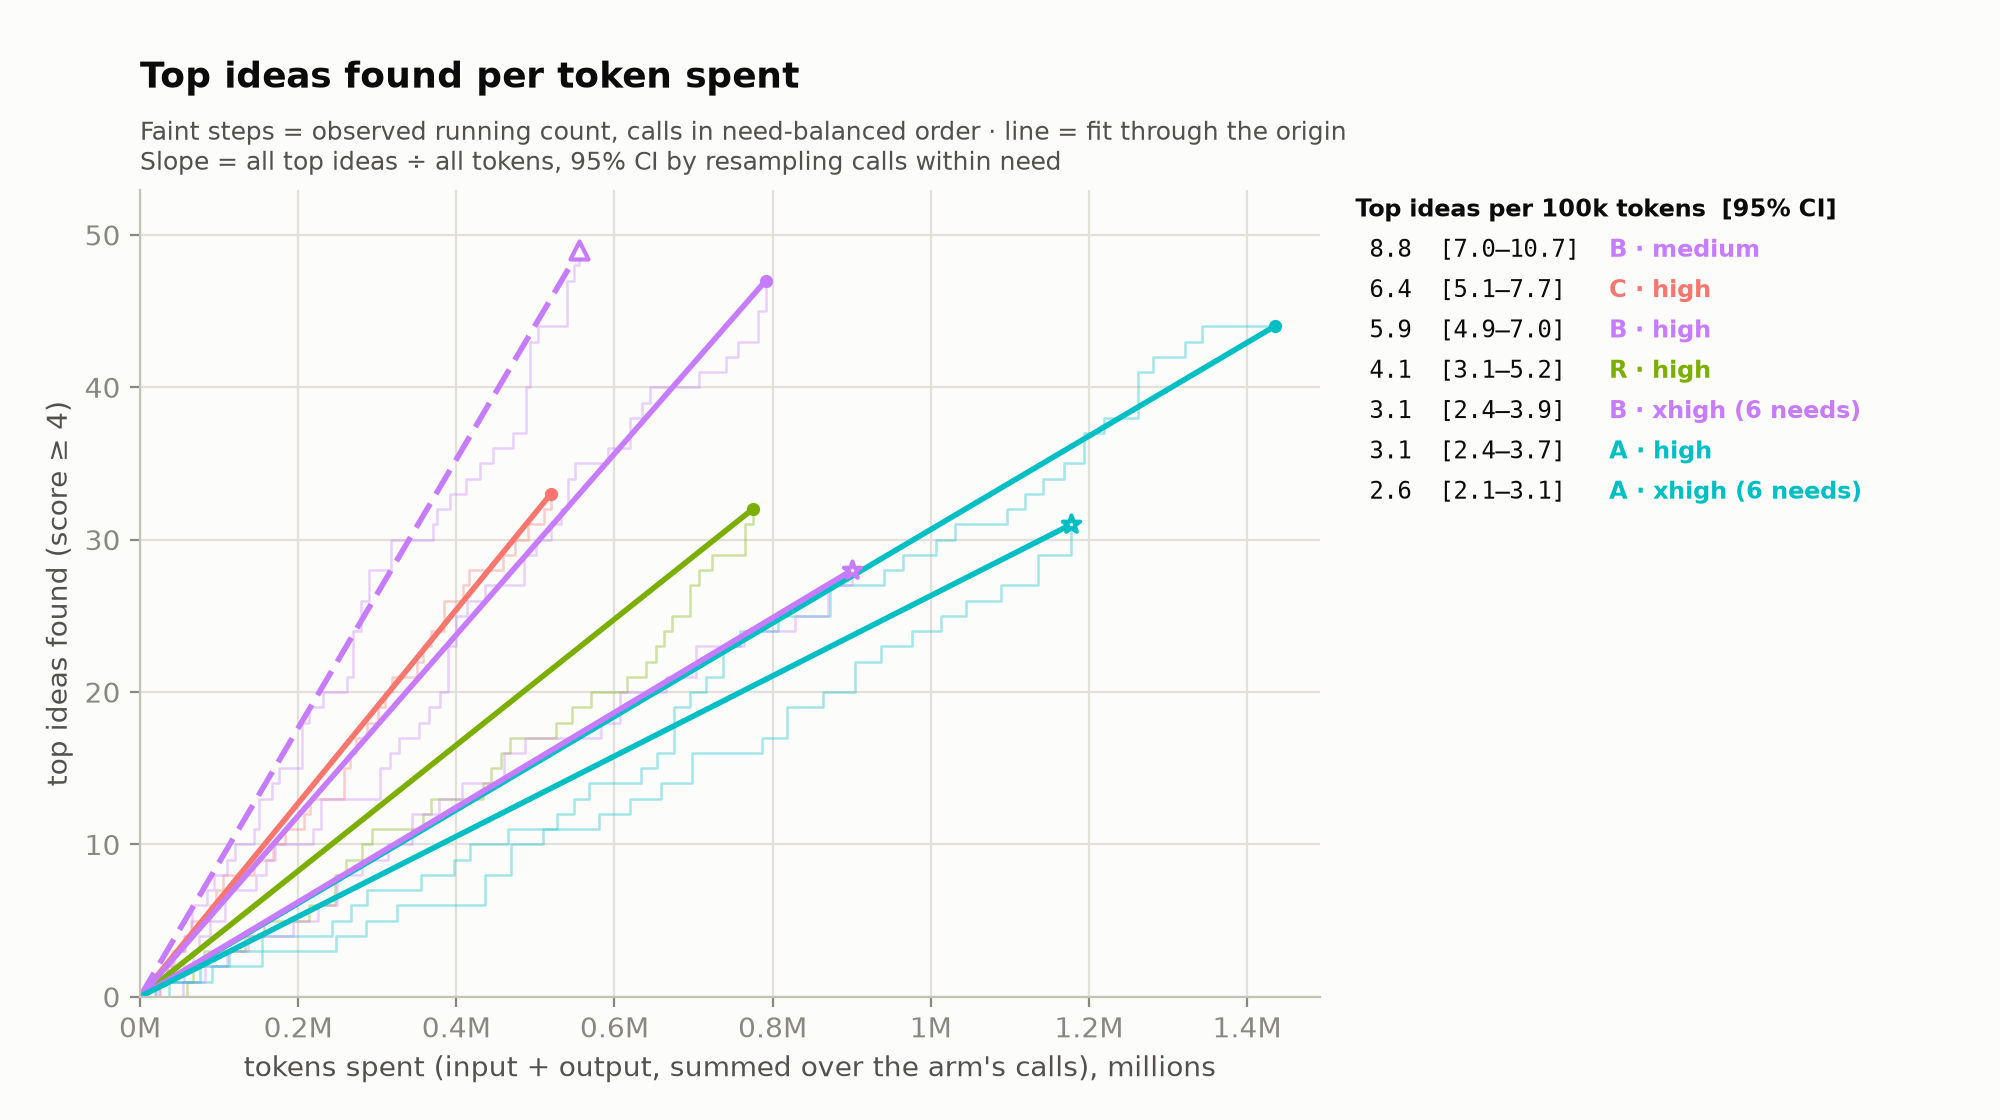
\includegraphics[width=\textwidth]{figures/8_top_ideas_vs_tokens.png}}{\fbox{\parbox[c][5cm][c]{0.9\textwidth}{\centering\small missing: \texttt{\detokenize{figures/8_top_ideas_vs_tokens.png}}}}}
\caption{Top ideas (score $\geq$ 4.0) found against tokens spent, per arm, with calls taken in replicate order. Each arm accumulates top ideas at a near-constant rate, so its slope is its yield (top ideas per 100k tokens): the steeper the line, the more efficient the arm. The market-need slice at medium effort climbs fastest; the full-graph arms are the flattest at every effort.}
\label{fig:yield}
\end{figure}

\begin{figure}[tbp]
\centering
\IfFileExists{figures/8c_yield_spread_annotated.png}{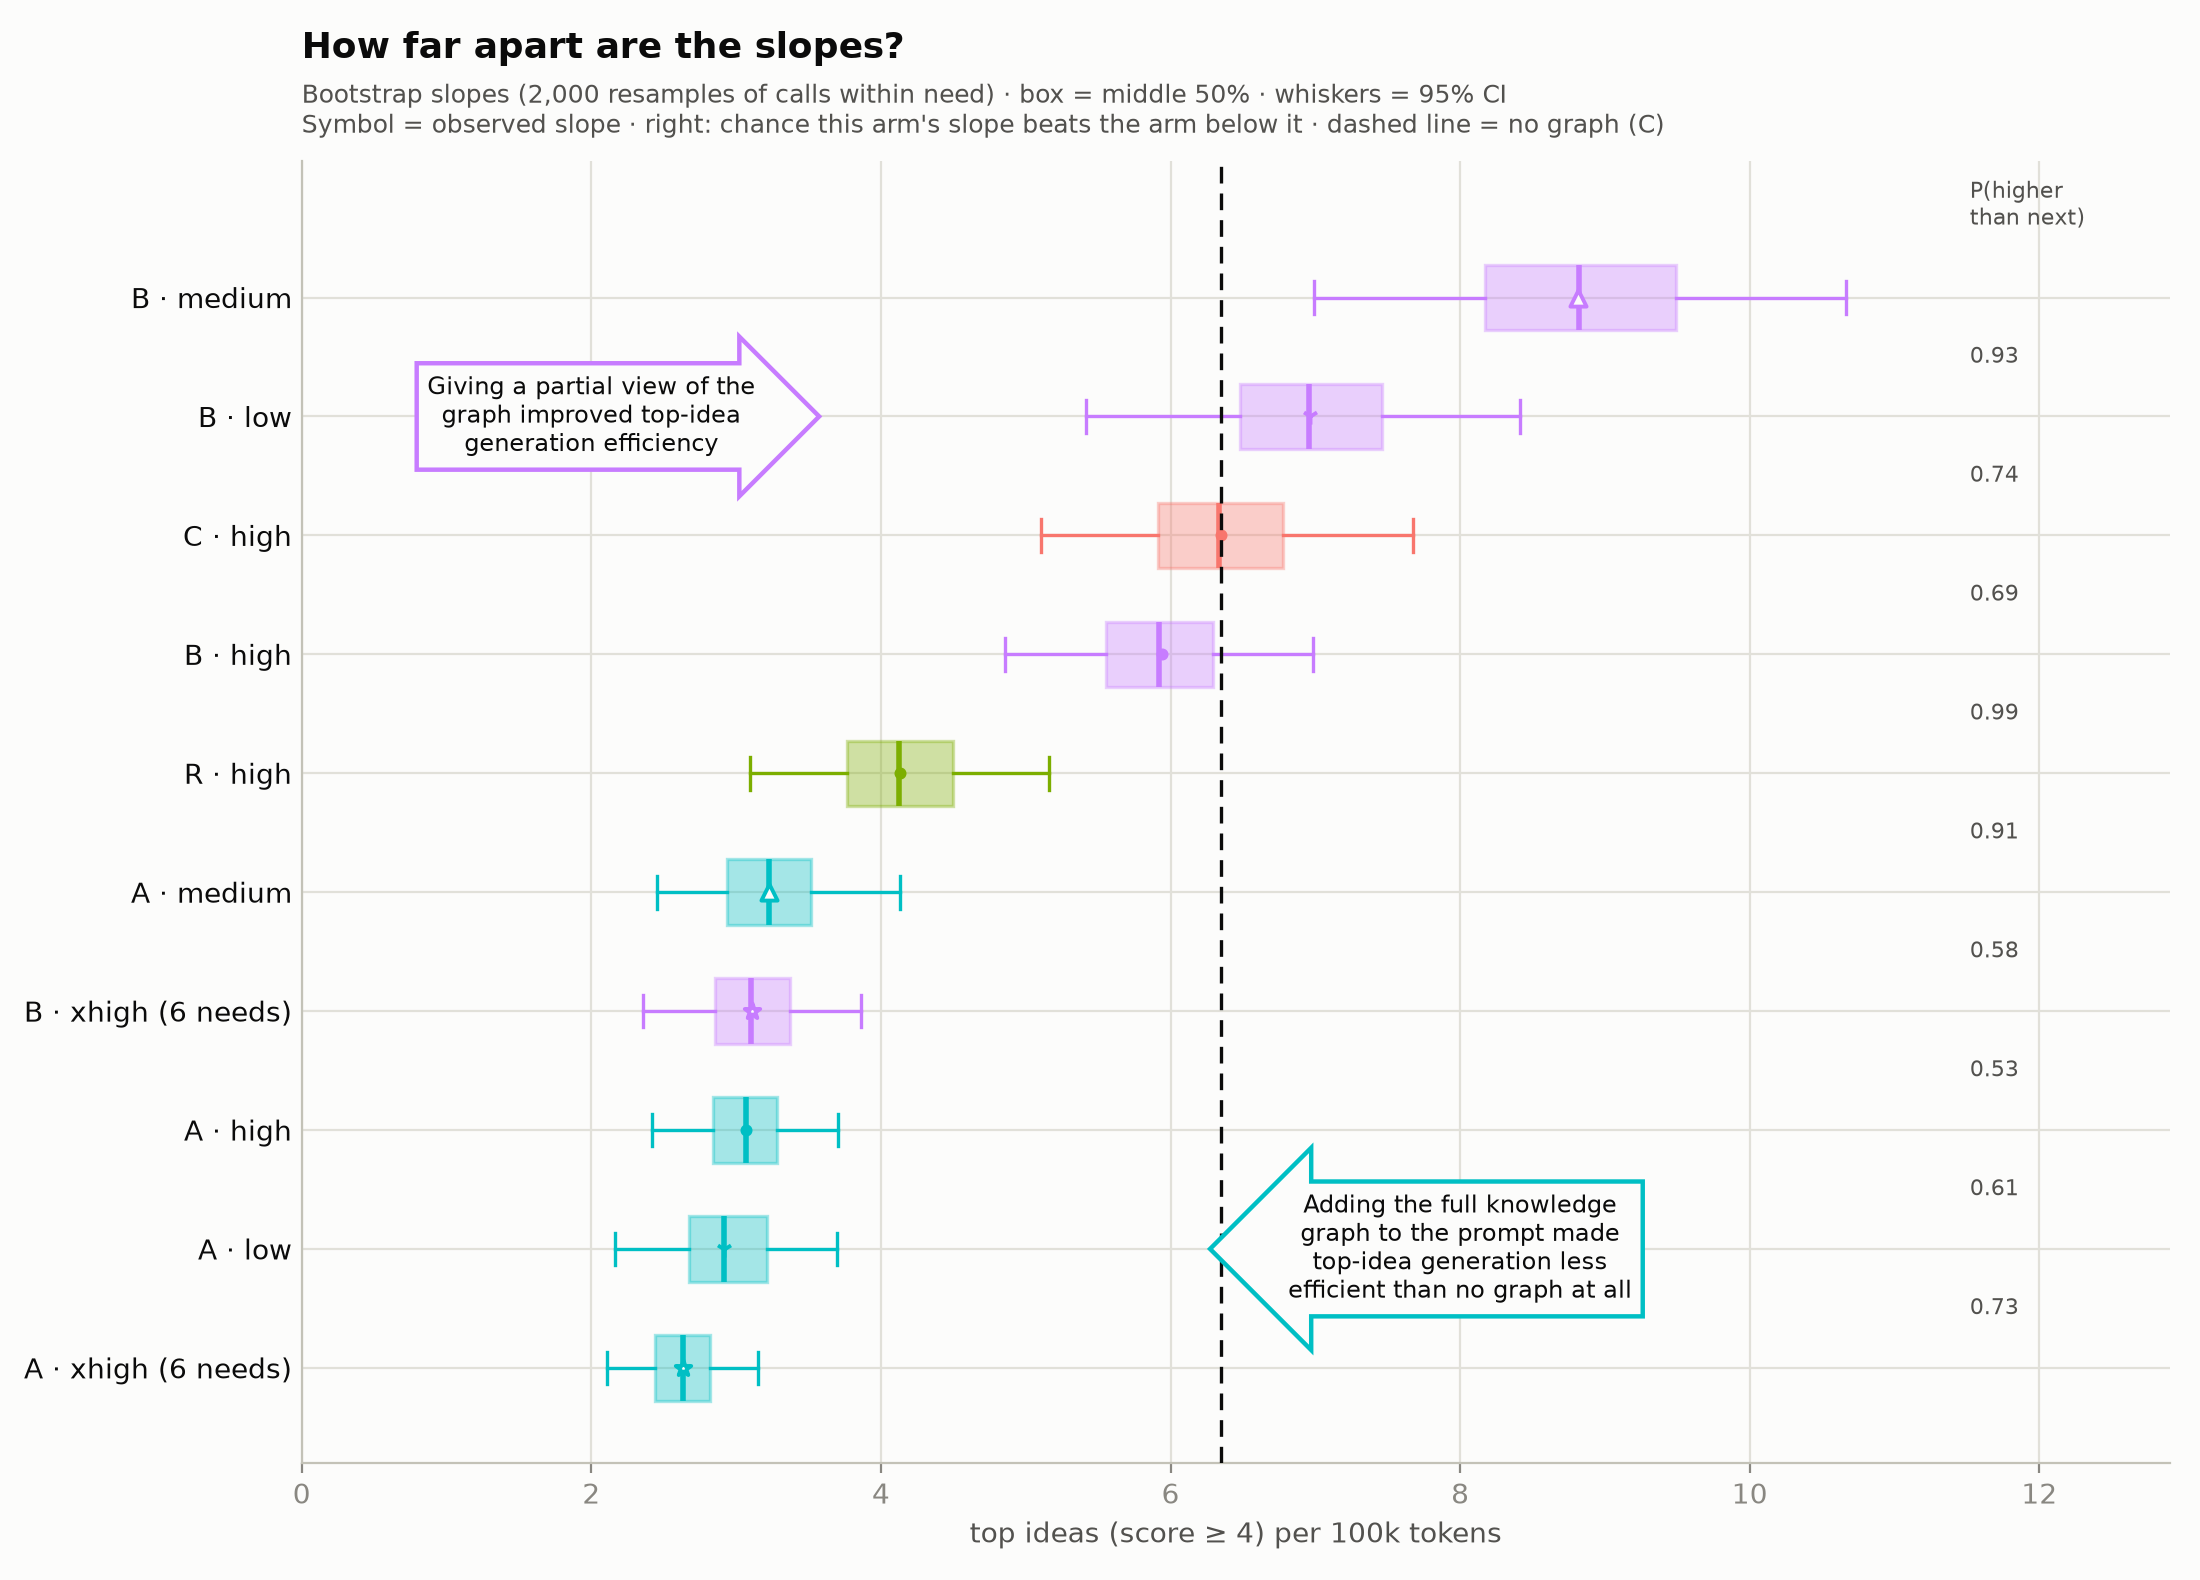
\includegraphics[width=\textwidth]{figures/8c_yield_spread_annotated.png}}{\fbox{\parbox[c][5cm][c]{0.9\textwidth}{\centering\small missing: \texttt{\detokenize{figures/8c_yield_spread_annotated.png}}}}}
\caption{How certain the yields are: for each arm, a box plot of 2,000 bootstrap slopes (calls resampled within market need; box = middle 50\%, whiskers = 95\% interval). The dashed line marks the control, no knowledge graph in the prompt (C, high effort). Arms whose boxes lie to the left of the line find top ideas less efficiently than giving the model no graph at all; this includes every full-graph arm, the random slice, and the market-need slice at high and extra-high effort (high only marginally). Only the market-need slice at low and medium effort lies to the right, more efficient than no graph.}
\label{fig:spread}
\end{figure}

The top-idea rate says how good an arm's ideas are; the yield says how fast it finds top ideas for the money. Counting top ideas against the tokens spent on an arm's calls (taken in replicate order, cycling through the market needs) gives a running count that grows in a straight line for every arm (Figure \ref{fig:yield}). The \textbf{yield} is the slope of that line: all of the arm's top ideas divided by all its tokens, per 100k tokens, with a 95\% CI from 2,000 resamples of calls within each market need. Unlike a probability, a count does not level off, so arms are compared directly by slope.

\begin{longtable}[]{@{}
  >{\raggedright\arraybackslash}p{(\columnwidth - 8\tabcolsep) * \real{0.4000}}
  >{\raggedright\arraybackslash}p{(\columnwidth - 8\tabcolsep) * \real{0.0769}}
  >{\raggedright\arraybackslash}p{(\columnwidth - 8\tabcolsep) * \real{0.1077}}
  >{\raggedright\arraybackslash}p{(\columnwidth - 8\tabcolsep) * \real{0.2923}}
  >{\raggedright\arraybackslash}p{(\columnwidth - 8\tabcolsep) * \real{0.1231}}@{}}
\toprule\noalign{}
\begin{minipage}[b]{\linewidth}\raggedright
Arm
\end{minipage} & \begin{minipage}[b]{\linewidth}\raggedright
Top ideas
\end{minipage} & \begin{minipage}[b]{\linewidth}\raggedright
Tokens spent
\end{minipage} & \begin{minipage}[b]{\linewidth}\raggedright
Yield (top ideas per 100k tokens)
\end{minipage} & \begin{minipage}[b]{\linewidth}\raggedright
95\% CI
\end{minipage} \\
\midrule\noalign{}
\endhead
\bottomrule\noalign{}
\endlastfoot
B · medium & 49 & 0.56M & \textbf{8.8} & 7.0--10.7 \\
B · low & 30 & 0.43M & 7.0 & 5.4--8.4 \\
C · high & 33 & 0.52M & 6.4 & 5.1--7.7 \\
B · high & 47 & 0.79M & 5.9 & 4.9--7.0 \\
R · high & 32 & 0.77M & 4.1 & 3.1--5.2 \\
A · medium & 34 & 1.05M & 3.2 & 2.5--4.1 \\
B · xhigh (6 market needs) & 28 & 0.90M & 3.1 & 2.4--3.9 \\
A · high & 44 & 1.43M & 3.1 & 2.4--3.7 \\
A · low & 27 & 0.93M & 2.9 & 2.2--3.7 \\
A · xhigh (6 market needs) & 31 & 1.18M & 2.6 & 2.1--3.1 \\
\end{longtable}

\begin{itemize}
\tightlist
\item
  \textbf{The market-need slice is the most efficient representation at every effort up to high.} B at medium yields 8.8 top ideas per 100k tokens, 2.8 times A at medium (3.2); at high, 5.9 against 3.1. The intervals do not overlap.
\item
  \textbf{The full graph's yield is flat across effort} (2.6--3.2). More thinking raises A's top-idea rate from 8\% to 21\%, but the cost per call rises in step, so the full graph buys better calls, not more top ideas per token.
\item
  \textbf{The slice's yield peaks at medium effort.} From medium to high, B's top-idea rate barely changes (15.1\% to 14.7\%) while the tokens per call rise by 45\%; xhigh raises the rate to 18.7\% but at 3.5 times the tokens.
\item
  \textbf{Relevance vs size:} at high effort, B yields 5.9 and R 4.1; the 95\% intervals just touch (4.9--7.0 against 3.1--5.2), but pairing the two arms' bootstrap draws, B's slope is the higher in 99\% of them (Figure \ref{fig:spread}), equivalent to a one-sided bootstrap p ≈ 0.01. R costs about as much per call as B, so the difference is in what the calls find.
\item
  \textbf{How far apart the slopes are} (Figure \ref{fig:spread}, chance that each arm's slope beats the next lower arm's): B·medium over B·low 0.93; B·low over C 0.74; C over B·high 0.69; B·high over R 0.99; R over A·medium 0.91; among the full-graph arms and B·xhigh 0.53--0.73. Four tiers: B at medium (8.8); B at low and high with C (5.9--7.0); R (4.1); all full-graph arms and B·xhigh (2.6--3.2).
\item
  \textbf{No graph:} C's low top-idea rate (10.2\%) is offset by its cheap calls (8.0k tokens), giving a yield of 6.4, above R and A and within the interval of B at high effort. Its weakness is coverage: with no graph, M1 produced no top idea in 5 calls (A and B: 2--3).
\item
  \textbf{At the stricter threshold (≥ 4.25)} the order is similar but the counts are small (2--11 per arm): B·medium 1.8 per 100k tokens (1.1--2.7), A·medium 1.0, B·low 0.9, B·high 0.9, A·xhigh 0.85, B·xhigh 0.8, C 0.8, A·high 0.7, R 0.4, A·low 0.2.
\item
  \textbf{On the 6 xhigh market needs only:} B·medium 9.0, B·low 7.4, B·high 6.4, C 6.1, R 4.2, A·low 3.3, B·xhigh 3.1, A·medium 2.9, A·high 2.8, A·xhigh 2.6. The ranking is the same as on all market needs.
\end{itemize}

\hypertarget{yield-per-market-need}{%
\subsubsection{Yield per market need}\label{yield-per-market-need}}

\begin{figure}[tbp]
\centering
\IfFileExists{figures/9_slice_size_effect.png}{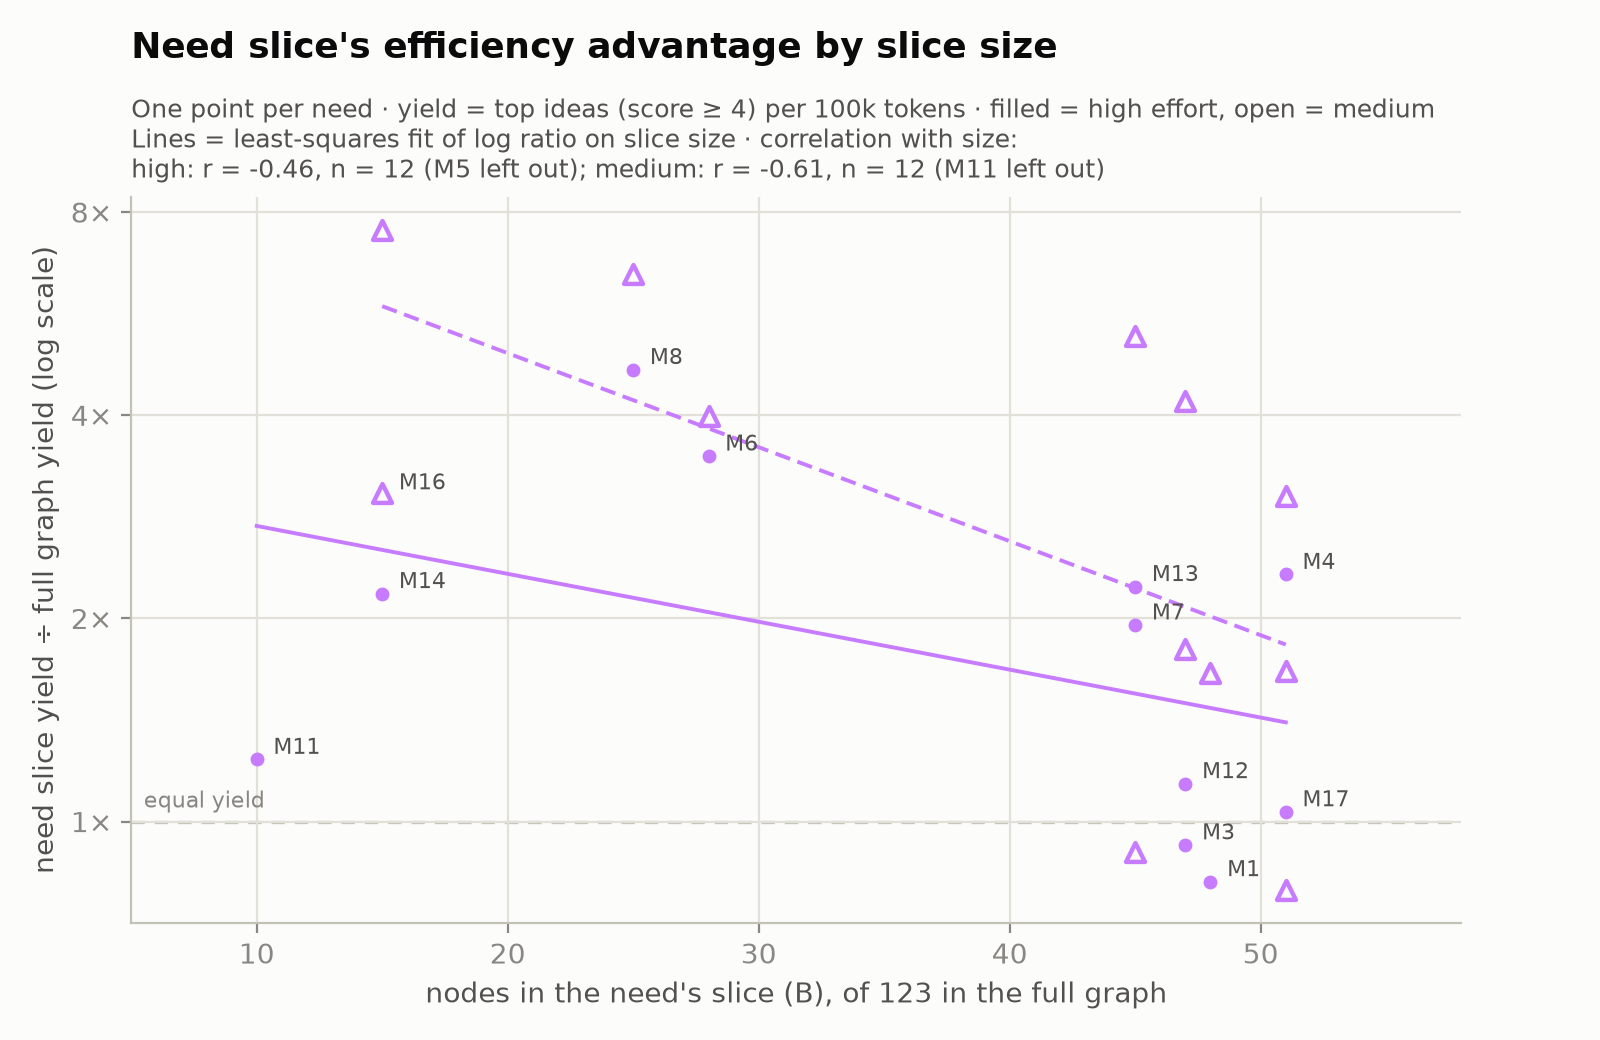
\includegraphics[width=\textwidth]{figures/9_slice_size_effect.png}}{\fbox{\parbox[c][5cm][c]{0.9\textwidth}{\centering\small missing: \texttt{\detokenize{figures/9_slice_size_effect.png}}}}}
\caption{Per market need: the market-need slice's yield divided by the full graph's, against the number of nodes in the slice (log scale; market needs with zero yield omitted).}
\label{fig:slicesize}
\end{figure}

To check that the yield ranking is not driven by a few easy market needs, yields were computed for each market need separately (5 calls per arm and market need), and arms were compared by the number of needs on which each is more efficient (exact two-sided sign test, ties excluded; \texttt{yield\_per\_market\_need.xlsx}).

Yield per market need at high effort (top ideas per 100k tokens; B's slice size in nodes):

\begin{longtable}[]{@{}
  >{\raggedright\arraybackslash}p{(\columnwidth - 12\tabcolsep) * \real{0.0667}}
  >{\raggedright\arraybackslash}p{(\columnwidth - 12\tabcolsep) * \real{0.1333}}
  >{\raggedright\arraybackslash}p{(\columnwidth - 12\tabcolsep) * \real{0.2444}}
  >{\raggedright\arraybackslash}p{(\columnwidth - 12\tabcolsep) * \real{0.1333}}
  >{\raggedright\arraybackslash}p{(\columnwidth - 12\tabcolsep) * \real{0.1778}}
  >{\raggedright\arraybackslash}p{(\columnwidth - 12\tabcolsep) * \real{0.1556}}
  >{\raggedright\arraybackslash}p{(\columnwidth - 12\tabcolsep) * \real{0.0889}}@{}}
\toprule\noalign{}
\begin{minipage}[b]{\linewidth}\raggedright
Need
\end{minipage} & \begin{minipage}[b]{\linewidth}\raggedright
Slice nodes
\end{minipage} & \begin{minipage}[b]{\linewidth}\raggedright
B market-need slice
\end{minipage} & \begin{minipage}[b]{\linewidth}\raggedright
C no graph
\end{minipage} & \begin{minipage}[b]{\linewidth}\raggedright
R random slice
\end{minipage} & \begin{minipage}[b]{\linewidth}\raggedright
A full graph
\end{minipage} & \begin{minipage}[b]{\linewidth}\raggedright
B ÷ A
\end{minipage} \\
\midrule\noalign{}
\endhead
\bottomrule\noalign{}
\endlastfoot
M11 & 10 & 2.1 & 0.0 & 2.1 & 1.7 & 1.2× \\
M14 & 15 & 17.9 & 15.5 & 10.6 & 8.2 & 2.2× \\
M16 & 15 & 9.2 & 5.1 & 2.5 & 3.0 & 3.1× \\
M8 & 25 & 13.4 & 10.1 & 7.6 & 2.9 & 4.7× \\
M6 & 28 & 11.8 & 7.4 & 5.8 & 3.4 & 3.5× \\
M7 & 45 & 5.5 & 12.8 & 5.8 & 2.8 & 2.0× \\
M13 & 45 & 6.0 & 5.0 & 3.1 & 2.7 & 2.2× \\
M3 & 47 & 4.1 & 10.0 & 4.8 & 4.5 & 0.9× \\
M12 & 47 & 3.1 & 2.6 & 1.6 & 2.8 & 1.1× \\
M1 & 48 & 2.6 & 0.0 & 0.0 & 3.2 & 0.8× \\
M4 & 51 & 4.3 & 6.8 & 4.1 & 1.9 & 2.3× \\
M5 & 51 & 0.0 & 0.0 & 1.5 & 0.0 & --- \\
M17 & 51 & 2.9 & 7.9 & 6.1 & 2.8 & 1.0× \\
\end{longtable}

\begin{longtable}[]{@{}
  >{\raggedright\arraybackslash}p{(\columnwidth - 8\tabcolsep) * \real{0.4783}}
  >{\raggedright\arraybackslash}p{(\columnwidth - 8\tabcolsep) * \real{0.2174}}
  >{\raggedright\arraybackslash}p{(\columnwidth - 8\tabcolsep) * \real{0.1739}}
  >{\raggedright\arraybackslash}p{(\columnwidth - 8\tabcolsep) * \real{0.0435}}
  >{\raggedright\arraybackslash}p{(\columnwidth - 8\tabcolsep) * \real{0.0870}}@{}}
\toprule\noalign{}
\begin{minipage}[b]{\linewidth}\raggedright
Comparison
\end{minipage} & \begin{minipage}[b]{\linewidth}\raggedright
First arm more efficient
\end{minipage} & \begin{minipage}[b]{\linewidth}\raggedright
Second more efficient
\end{minipage} & \begin{minipage}[b]{\linewidth}\raggedright
Equal
\end{minipage} & \begin{minipage}[b]{\linewidth}\raggedright
Sign test p
\end{minipage} \\
\midrule\noalign{}
\endhead
\bottomrule\noalign{}
\endlastfoot
B vs A, high effort & 10 market needs & 2 & 1 & \textbf{0.039} \\
B vs A, medium effort & 10 & 3 & 0 & 0.092 \\
C vs R (no graph vs random slice) & 10 & 2 & 1 & \textbf{0.039} \\
R vs A & 10 & 3 & 0 & 0.092 \\
C vs A & 9 & 3 & 1 & 0.146 \\
B vs R & 9 & 4 & 0 & 0.267 \\
B vs C & 8 & 4 & 1 & 0.388 \\
\end{longtable}

\begin{itemize}
\tightlist
\item
  \textbf{The slice's efficiency advantage over the full graph holds market need by market need:} B is more efficient on 10 of 13 market needs at high effort (p = 0.039) and at medium effort (p = 0.09). The full graph is ahead only on M1 and M3, by small margins.
\item
  \textbf{No graph is more efficient than a random slice on 10 of 12 decided market needs (p = 0.039).} Showing the model structure that is not about the problem costs more per top idea than showing it nothing.
\item
  \textbf{Relevance vs size (B vs R) is not robust market need by market need} (9 of 13, p = 0.27), in line with the pooled yield (intervals touching) and the set judging (no difference).
\item
  \textbf{The advantage depends on slice size (exploratory).} B's lead over A is largest where the slice is small: 3--5× for M6, M8 and M16 (15--28 nodes), against 0.8--2.3× for the market needs with 45--51 nodes (Figure \ref{fig:slicesize}). Across market needs, the log of B's yield ratio over A correlates with slice size at r = −0.46 at high effort (n = 12, p ≈ 0.13) and r = −0.61 at medium effort (n = 12, p ≈ 0.04). M11, the smallest slice (10 nodes), is an exception at 1.2×; it is also one of the two hardest market needs for every arm. A smaller slice saves more tokens and is more focused; with 13 market needs and 5 calls each this is a pattern to test, not an established result.
\item
  \textbf{Single needs are noisy:} each value rests on 5 calls and 0--10 top ideas.
\end{itemize}

\hypertarget{chance-of-at-least-one-top-idea-for-a-given-budget-secondary}{%
\subsubsection{Chance of at least one top idea for a given budget (secondary)}\label{chance-of-at-least-one-top-idea-for-a-given-budget-secondary}}

\begin{figure}[tbp]
\centering
\IfFileExists{figures/7_chance_vs_budget.png}{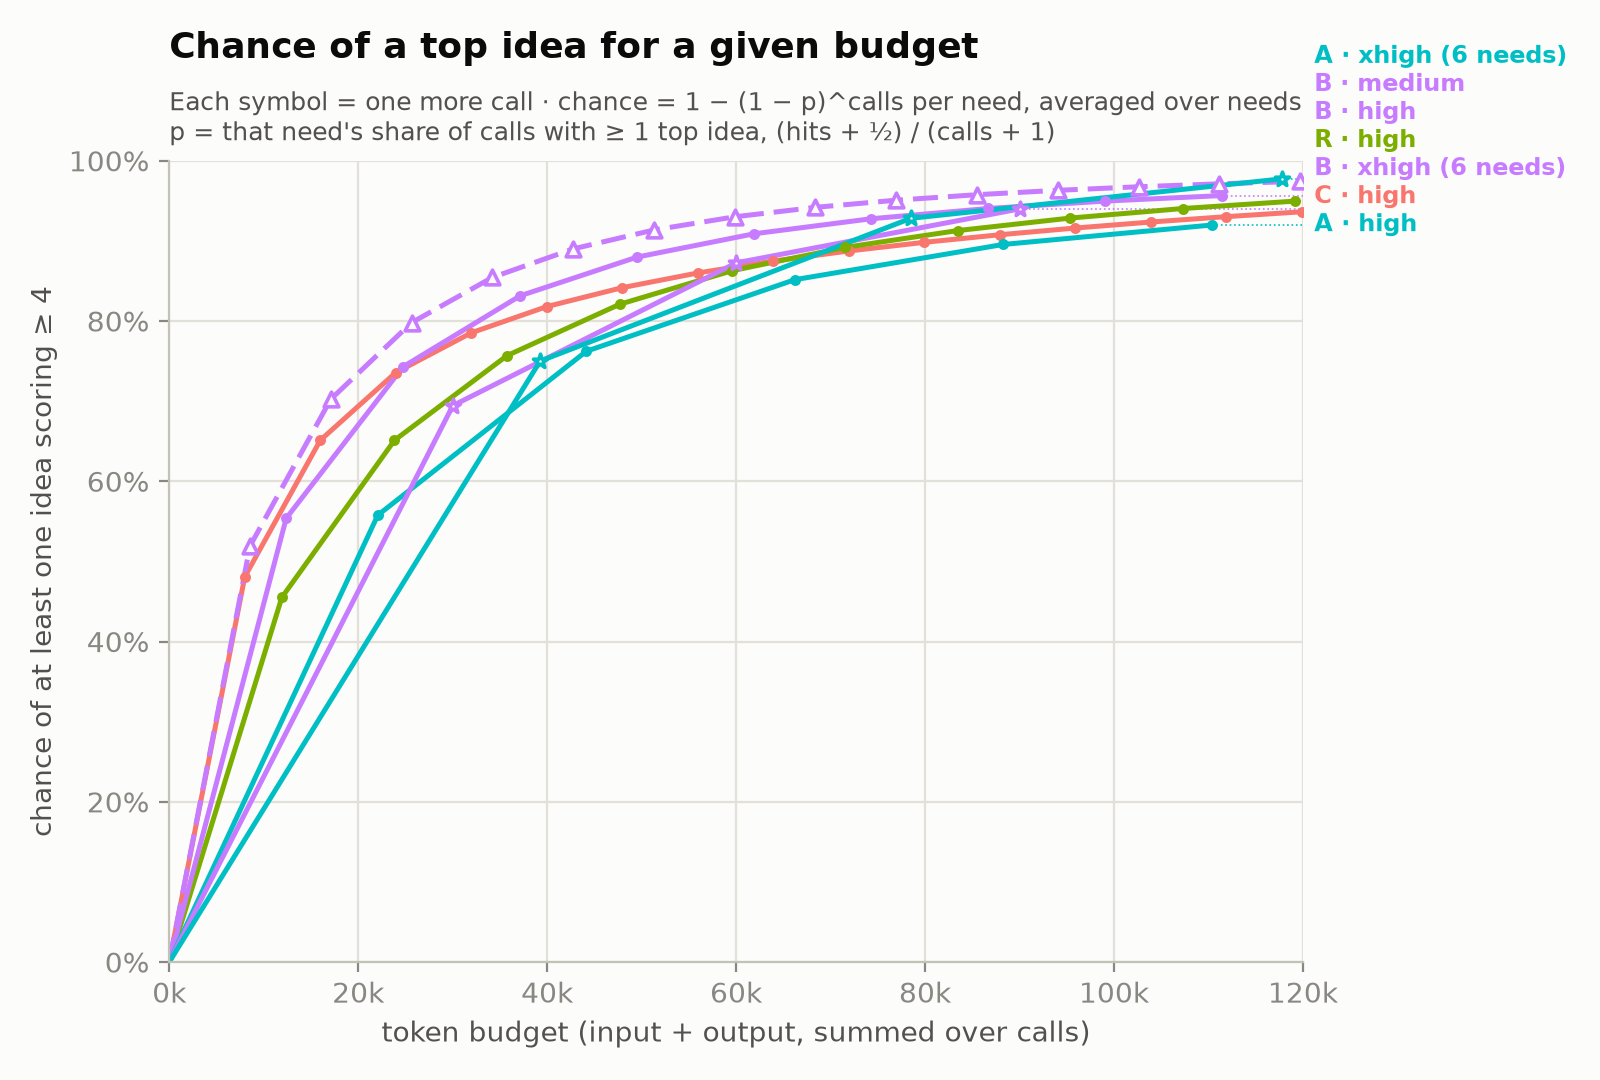
\includegraphics[width=\textwidth]{figures/7_chance_vs_budget.png}}{\fbox{\parbox[c][5cm][c]{0.9\textwidth}{\centering\small missing: \texttt{\detokenize{figures/7_chance_vs_budget.png}}}}}
\caption{Chance of at least one top idea for a given token budget, per arm, from whole calls and a Jeffreys estimate of each market need's success rate. Every curve rises towards 1 as the budget grows, so this view compresses differences at large budgets; yield (Figure \ref{fig:yield}) is the main measure.}
\label{fig:budget}
\end{figure}

Figure \ref{fig:budget} shows the curves.

This measure answers a practical question, how likely one budget is to produce at least one top idea, but every arm's chance approaches 100\% as the budget grows, so it compresses differences at large budgets and can suggest that spending alone guarantees a top idea. The yield above is the better basis for comparing arms. For a token budget spent on whole calls of one arm, the chance that at least one idea scores ≥ 4.0, averaged over market needs. Within a market need, calls are treated as independent: k calls succeed with 1 − (1 − p)\^{}k, where p is the market need's share of calls with a top idea, estimated as (hits + ½) / (calls + 1) because 5 calls per market need often give exactly 0 or 1.

\begin{longtable}[]{@{}llll@{}}
\toprule\noalign{}
Arm & 25k tokens & 50k tokens & 100k tokens \\
\midrule\noalign{}
\endhead
\bottomrule\noalign{}
\endlastfoot
C · high & 74\% (3 calls) & 84\% (6) & 92\% (12) \\
R · high & 65\% (2) & 82\% (4) & 93\% (8) \\
B · low & 64\% (3) & 81\% (7) & 91\% (15) \\
B · medium & 70\% (2) & \textbf{89\%} (5) & \textbf{96\%} (11) \\
B · high & 74\% (2) & 88\% (4) & 95\% (8) \\
B · xhigh (6 market needs) & --- (0) & 69\% (1) & 94\% (3) \\
A · low & 39\% (1) & 67\% (3) & 86\% (7) \\
A · medium & 46\% (1) & 79\% (3) & 94\% (6) \\
A · high & 56\% (1) & 76\% (2) & 90\% (4) \\
A · xhigh (6 market needs) & --- (0) & 75\% (1) & 93\% (2) \\
\end{longtable}

\begin{itemize}
\tightlist
\item
  \textbf{B at medium and high effort lead at 50k and 100k tokens,} and B-medium is at or near the top at every budget.
\item
  \textbf{No graph is a good choice for small budgets} because its calls are cheapest, but it rises more slowly at large budgets because of the market needs where it finds nothing (M1); M5 and M11 are hard for every arm.
\item
  \textbf{The full graph trails at every budget:} its calls are expensive and its top-idea rate is no higher than B's.
\end{itemize}

\hypertarget{stricter-threshold-and-matched-market-needs}{%
\subsubsection{Stricter threshold and matched market needs}\label{stricter-threshold-and-matched-market-needs}}

\begin{itemize}
\tightlist
\item
  \textbf{Score ≥ 4.25 (top 2.4\%):} same direction, too few hits per arm (2--11) to separate arms. A·xhigh 6.7\% and B·xhigh 4.7\% (6 market needs), A·medium 3.4\%, B·medium 3.1\%, A·high 3.1\%, B·high 2.2\%, C 1.2\%, B·low 1.2\%, R 1.0\%, A·low 0.6\%. Tokens per top idea are lowest for B·medium (56k) and highest for R (about 260k) and A·low (463k); yields are listed in the yield section above.
\item
  \textbf{Only the 6 xhigh market needs} (\texttt{-\/-match-needs}): B·medium and B·high 16.7\%, B·xhigh 18.7\%, A·high 12.7\%, A·xhigh 20.7\%, R 10.7\%, C 10.0\%. On equal market needs, B gains little from xhigh over medium or high, while A gains a lot; A needs the extra thinking to make use of its larger context.
\end{itemize}

\hypertarget{mean-idea-quality-individual-scoring}{%
\subsection{Mean idea quality (individual scoring)}\label{mean-idea-quality-individual-scoring}}

\begin{figure}[tbp]
\centering
\IfFileExists{figures/4_cost_vs_quality.png}{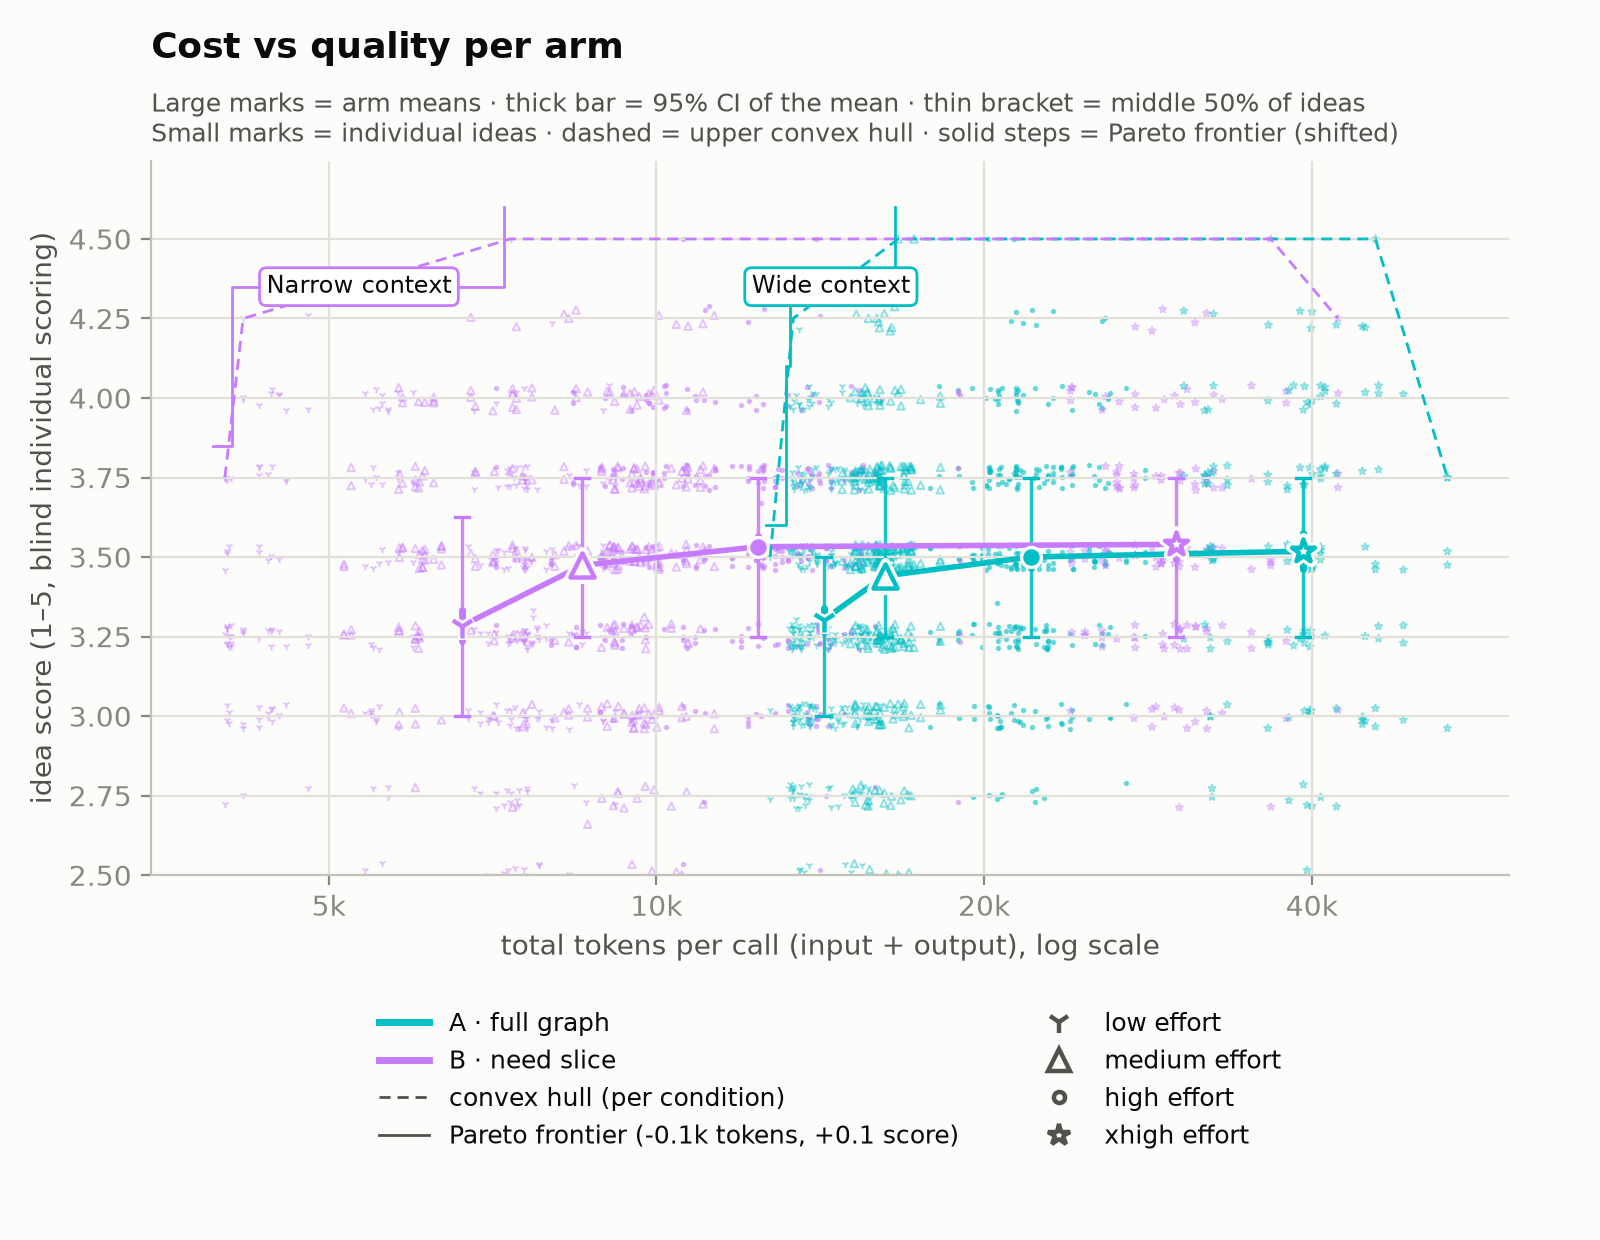
\includegraphics[width=\textwidth]{figures/4_cost_vs_quality.png}}{\fbox{\parbox[c][5cm][c]{0.9\textwidth}{\centering\small missing: \texttt{\detokenize{figures/4_cost_vs_quality.png}}}}}
\caption{Tokens per call against mean idea score for the full-graph (A) and market-need-slice (B) arms at each effort. Moving right costs tokens; moving up raises the average idea, not necessarily the number of top ideas.}
\label{fig:costquality}
\end{figure}

Figure \ref{fig:costquality} plots tokens per call against mean idea score for the full-graph and market-need-slice arms.

Need-balanced mean idea score (1--5) and mean criterion scores:

\begin{longtable}[]{@{}llllll@{}}
\toprule\noalign{}
Arm & Mean score & Relevance & Novelty & Feasibility & Specificity \\
\midrule\noalign{}
\endhead
\bottomrule\noalign{}
\endlastfoot
C · high & 3.44 & 3.49 & 3.29 & 3.21 & 3.78 \\
R · high & 3.46 & 3.44 & 3.16 & 3.37 & 3.88 \\
B · low & 3.28 & 3.38 & 3.01 & 3.26 & 3.50 \\
B · medium & 3.47 & 3.53 & 3.20 & 3.36 & 3.82 \\
B · high & 3.53 & 3.60 & 3.25 & 3.37 & 3.92 \\
B · xhigh (6 market needs) & 3.54 & 3.47 & 3.38 & 3.29 & 4.03 \\
A · low & 3.30 & 3.39 & 3.04 & 3.27 & 3.52 \\
A · medium & 3.44 & 3.42 & 3.10 & 3.42 & 3.83 \\
A · high & 3.50 & 3.46 & 3.20 & 3.45 & 3.89 \\
A · xhigh (6 market needs) & 3.52 & 3.42 & 3.33 & 3.29 & 4.03 \\
\end{longtable}

\begin{itemize}
\tightlist
\item
  Mean differences between arms are small (0.1--0.25 points) and hide the differences in the tail; this is why the tail is the main measure.
\item
  At high effort, mean scores order C 3.44 \textless{} R 3.46 \textless{} A 3.50 \textless{} B 3.53, the same ranking as the top-idea rates except that C and R, nearly tied on both measures, swap places.
\item
  \textbf{No graph gives the most novel but least feasible single ideas} at high effort: novelty 3.29 (highest at high effort) and feasibility 3.21 (lowest). Without the graph, ideas are less constrained by the actual product. Judged as sets, though, A and B are rated more novel than C (below): the individual novelty advantage of C does not survive a side-by-side comparison.
\item
  \textbf{Individual ideas vs whole sets:} B's ideas score at least as well as A's individually, yet A wins 64\% of set comparisons. A's advantage is at the level of the set (specificity, diversity), not in better single ideas.
\end{itemize}

\hypertarget{pairwise-set-judging-full-graph-vs-market-need-slice-equal-effort}{%
\subsection{Pairwise set judging: full graph vs market-need slice (equal effort)}\label{pairwise-set-judging-full-graph-vs-market-need-slice-equal-effort}}

\begin{figure}[tbp]
\centering
\IfFileExists{figures/2_win_rates.png}{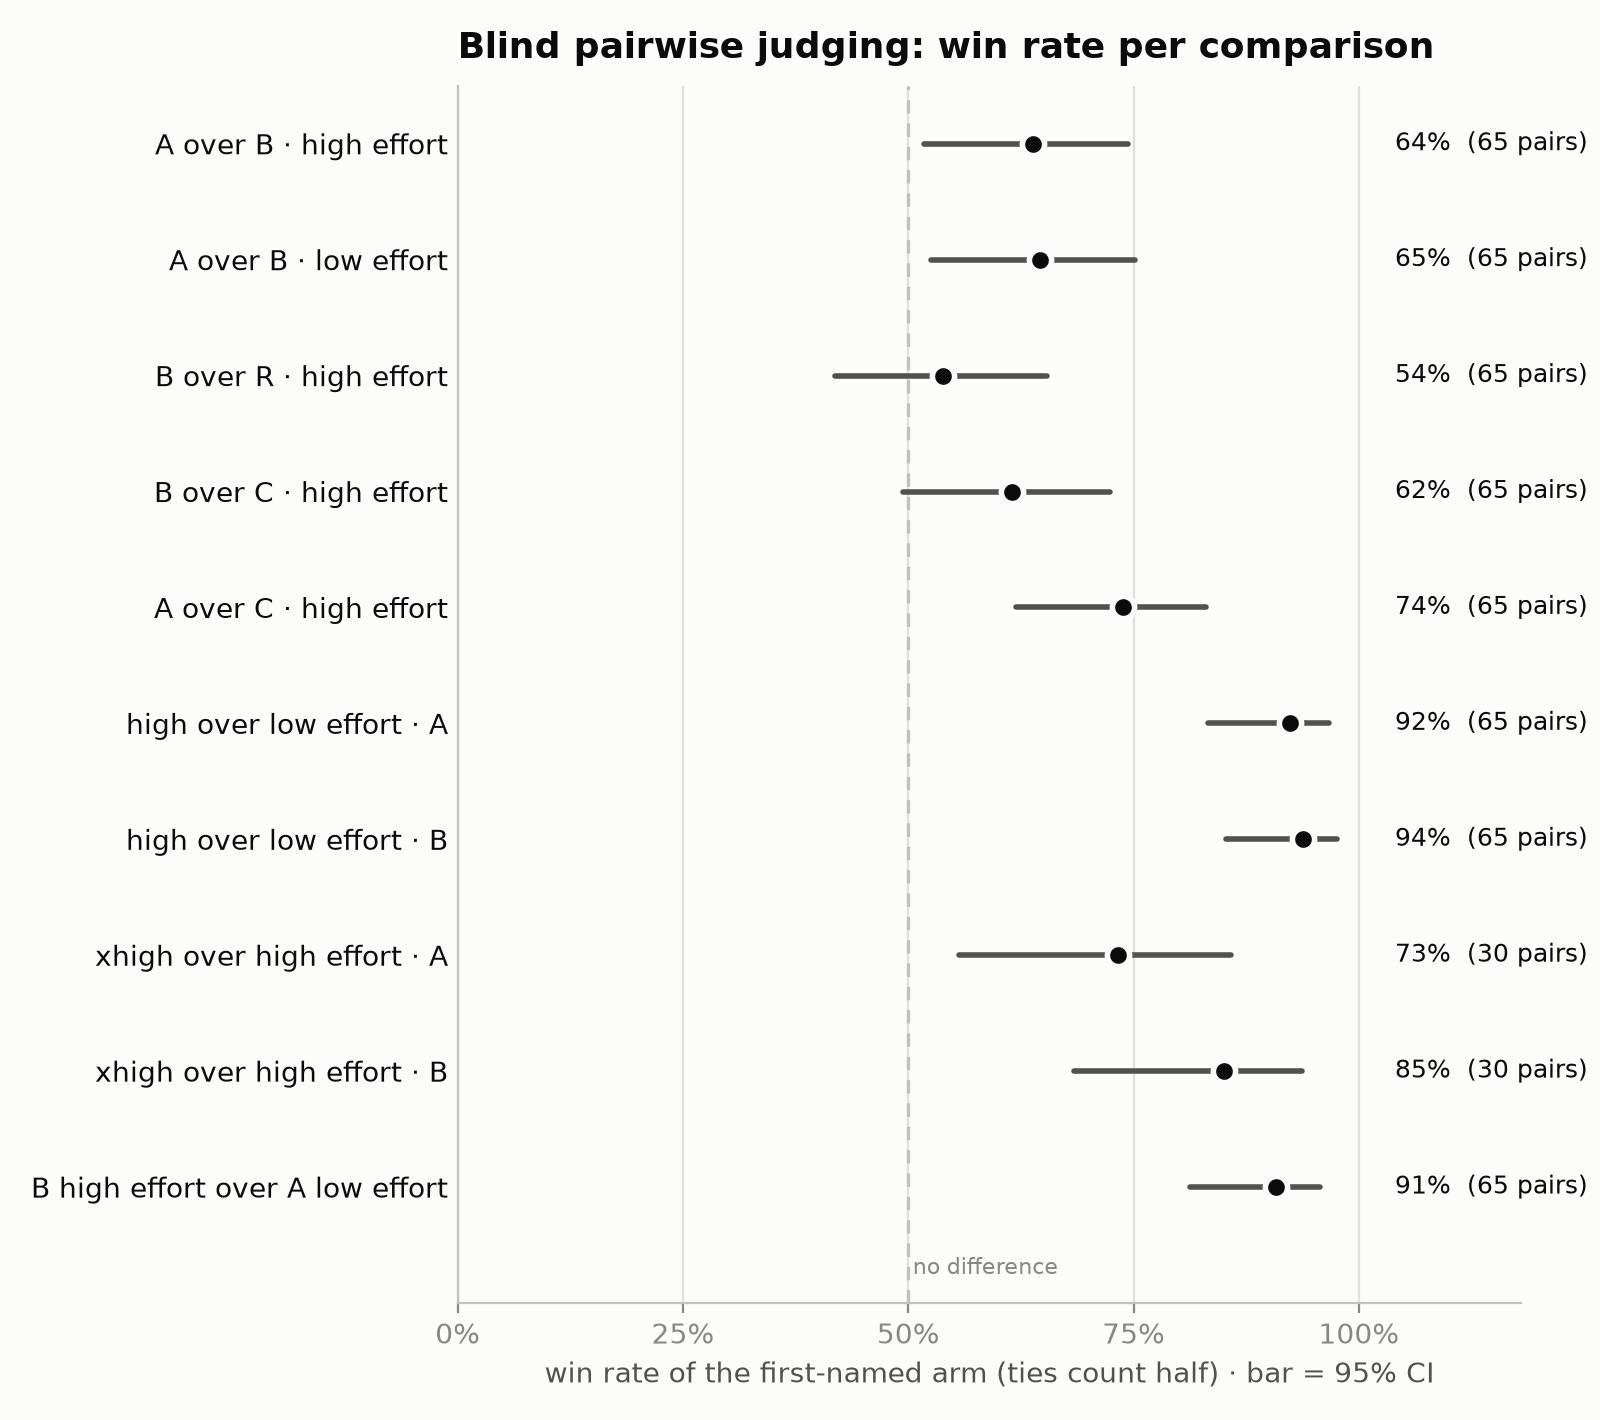
\includegraphics[width=\textwidth]{figures/2_win_rates.png}}{\fbox{\parbox[c][5cm][c]{0.9\textwidth}{\centering\small missing: \texttt{\detokenize{figures/2_win_rates.png}}}}}
\caption{Every pairwise set comparison: the first arm's win rate with a 95\% Wilson interval (each pair judged in both presentation orders, ties excluded). Values above 50\% favour the first arm.}
\label{fig:winrates}
\end{figure}

\begin{figure}[tbp]
\centering
\IfFileExists{figures/3_score_diff_A_minus_B.png}{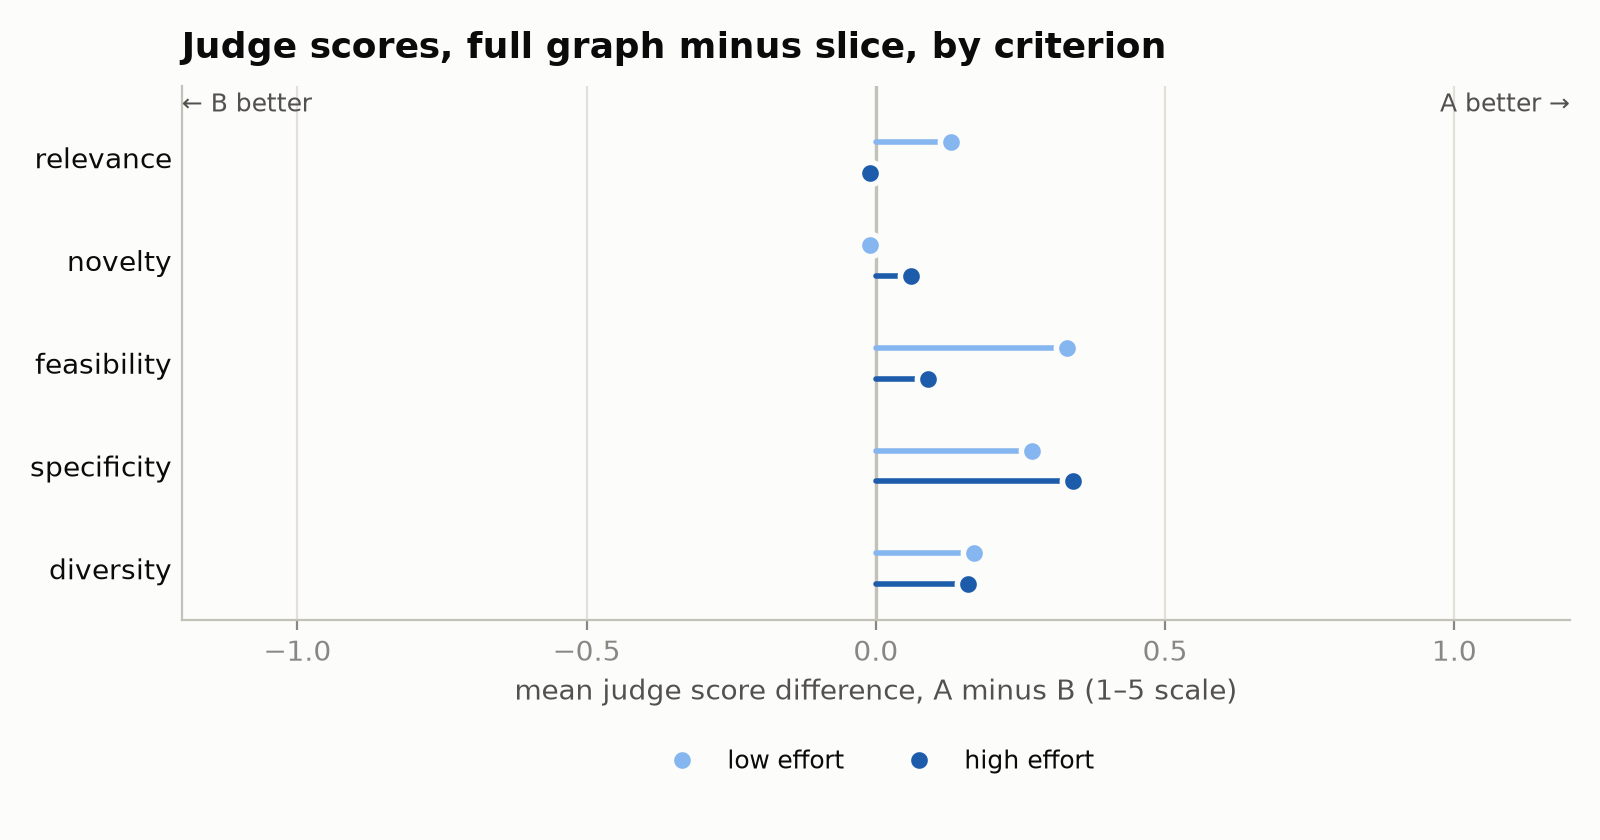
\includegraphics[width=\textwidth]{figures/3_score_diff_A_minus_B.png}}{\fbox{\parbox[c][5cm][c]{0.9\textwidth}{\centering\small missing: \texttt{\detokenize{figures/3_score_diff_A_minus_B.png}}}}}
\caption{Full graph minus market-need slice (A $-$ B) on each set-judging criterion, by effort. The full graph's advantage is mainly specificity.}
\label{fig:scorediff}
\end{figure}

Figure \ref{fig:winrates} shows every pairwise comparison in this and the next three sections; Figure \ref{fig:scorediff} shows how A and B differ on each criterion.

\begin{longtable}[]{@{}
  >{\raggedright\arraybackslash}p{(\columnwidth - 16\tabcolsep) * \real{0.0930}}
  >{\raggedright\arraybackslash}p{(\columnwidth - 16\tabcolsep) * \real{0.0698}}
  >{\raggedright\arraybackslash}p{(\columnwidth - 16\tabcolsep) * \real{0.0698}}
  >{\raggedright\arraybackslash}p{(\columnwidth - 16\tabcolsep) * \real{0.0698}}
  >{\raggedright\arraybackslash}p{(\columnwidth - 16\tabcolsep) * \real{0.0698}}
  >{\raggedright\arraybackslash}p{(\columnwidth - 16\tabcolsep) * \real{0.1395}}
  >{\raggedright\arraybackslash}p{(\columnwidth - 16\tabcolsep) * \real{0.1395}}
  >{\raggedright\arraybackslash}p{(\columnwidth - 16\tabcolsep) * \real{0.1395}}
  >{\raggedright\arraybackslash}p{(\columnwidth - 16\tabcolsep) * \real{0.2093}}@{}}
\toprule\noalign{}
\begin{minipage}[b]{\linewidth}\raggedright
Effort
\end{minipage} & \begin{minipage}[b]{\linewidth}\raggedright
Pairs
\end{minipage} & \begin{minipage}[b]{\linewidth}\raggedright
A wins
\end{minipage} & \begin{minipage}[b]{\linewidth}\raggedright
B wins
\end{minipage} & \begin{minipage}[b]{\linewidth}\raggedright
Ties
\end{minipage} & \begin{minipage}[b]{\linewidth}\raggedright
A win rate
\end{minipage} & \begin{minipage}[b]{\linewidth}\raggedright
95\% CI
\end{minipage} & \begin{minipage}[b]{\linewidth}\raggedright
Sign test p
\end{minipage} & \begin{minipage}[b]{\linewidth}\raggedright
Order agreement
\end{minipage} \\
\midrule\noalign{}
\endhead
\bottomrule\noalign{}
\endlastfoot
low & 65 & 37 & 18 & 10 & 65\% & 53--75\% & 0.015 & 85\% \\
high & 65 & 34 & 16 & 15 & 64\% & 52--74\% & 0.015 & 77\% \\
\end{longtable}

Mean score difference, A minus B (1--5 scale):

\begin{longtable}[]{@{}llllll@{}}
\toprule\noalign{}
Effort & Relevance & Novelty & Feasibility & Specificity & Diversity \\
\midrule\noalign{}
\endhead
\bottomrule\noalign{}
\endlastfoot
low & +0.13 & −0.01 & +0.33 & +0.27 & +0.17 \\
high & −0.01 & +0.06 & +0.09 & +0.34 & +0.16 \\
\end{longtable}

\begin{itemize}
\tightlist
\item
  The full graph's advantage on whole sets is real but modest, mainly in specificity; novelty and relevance are about equal.
\item
  \textbf{H2 (B no worse than A on sets) is rejected:} B's win rate is 35--36\%, with the lower confidence bound (25--26\%) well below the 45\% non-inferiority margin. On the tail measure, however, B is not worse than A at any effort.
\item
  \textbf{The effect varies by market need:} A swept 5--0 for M17 and M6 at high effort and M11 at low; B led for M1 at low effort, M3 at both levels and M8 at high. With 5 pairs per market need, no single market need is significant.
\end{itemize}

\hypertarget{pairwise-set-judging-the-controls-high-effort}{%
\subsection{Pairwise set judging: the controls (high effort)}\label{pairwise-set-judging-the-controls-high-effort}}

\begin{longtable}[]{@{}
  >{\raggedright\arraybackslash}p{(\columnwidth - 16\tabcolsep) * \real{0.4565}}
  >{\raggedright\arraybackslash}p{(\columnwidth - 16\tabcolsep) * \real{0.0326}}
  >{\raggedright\arraybackslash}p{(\columnwidth - 16\tabcolsep) * \real{0.0652}}
  >{\raggedright\arraybackslash}p{(\columnwidth - 16\tabcolsep) * \real{0.0652}}
  >{\raggedright\arraybackslash}p{(\columnwidth - 16\tabcolsep) * \real{0.0326}}
  >{\raggedright\arraybackslash}p{(\columnwidth - 16\tabcolsep) * \real{0.1087}}
  >{\raggedright\arraybackslash}p{(\columnwidth - 16\tabcolsep) * \real{0.0652}}
  >{\raggedright\arraybackslash}p{(\columnwidth - 16\tabcolsep) * \real{0.0761}}
  >{\raggedright\arraybackslash}p{(\columnwidth - 16\tabcolsep) * \real{0.0978}}@{}}
\toprule\noalign{}
\begin{minipage}[b]{\linewidth}\raggedright
Comparison
\end{minipage} & \begin{minipage}[b]{\linewidth}\raggedright
Pairs
\end{minipage} & \begin{minipage}[b]{\linewidth}\raggedright
First wins
\end{minipage} & \begin{minipage}[b]{\linewidth}\raggedright
Second wins
\end{minipage} & \begin{minipage}[b]{\linewidth}\raggedright
Ties
\end{minipage} & \begin{minipage}[b]{\linewidth}\raggedright
First-arm win rate
\end{minipage} & \begin{minipage}[b]{\linewidth}\raggedright
95\% CI
\end{minipage} & \begin{minipage}[b]{\linewidth}\raggedright
Sign test p
\end{minipage} & \begin{minipage}[b]{\linewidth}\raggedright
Order agreement
\end{minipage} \\
\midrule\noalign{}
\endhead
\bottomrule\noalign{}
\endlastfoot
A vs C (full graph vs no graph) & 65 & 44 & 13 & 8 & 74\% & 62--83\% & \textless{} 0.001 & 88\% \\
B vs C (market-need slice vs no graph) & 65 & 34 & 19 & 12 & 62\% & 49--72\% & 0.053 & 82\% \\
B vs R (market-need slice vs random slice) & 65 & 25 & 20 & 20 & 54\% & 42--65\% & 0.55 & 68\% \\
A vs B (for reference) & 65 & 34 & 16 & 15 & 64\% & 52--74\% & 0.015 & 77\% \\
\end{longtable}

Mean score difference, first minus second arm (1--5 scale):

\begin{longtable}[]{@{}
  >{\raggedright\arraybackslash}p{(\columnwidth - 10\tabcolsep) * \real{0.1818}}
  >{\raggedright\arraybackslash}p{(\columnwidth - 10\tabcolsep) * \real{0.1515}}
  >{\raggedright\arraybackslash}p{(\columnwidth - 10\tabcolsep) * \real{0.1515}}
  >{\raggedright\arraybackslash}p{(\columnwidth - 10\tabcolsep) * \real{0.1818}}
  >{\raggedright\arraybackslash}p{(\columnwidth - 10\tabcolsep) * \real{0.1818}}
  >{\raggedright\arraybackslash}p{(\columnwidth - 10\tabcolsep) * \real{0.1515}}@{}}
\toprule\noalign{}
\begin{minipage}[b]{\linewidth}\raggedright
Comparison
\end{minipage} & \begin{minipage}[b]{\linewidth}\raggedright
Relevance
\end{minipage} & \begin{minipage}[b]{\linewidth}\raggedright
Novelty
\end{minipage} & \begin{minipage}[b]{\linewidth}\raggedright
Feasibility
\end{minipage} & \begin{minipage}[b]{\linewidth}\raggedright
Specificity
\end{minipage} & \begin{minipage}[b]{\linewidth}\raggedright
Diversity
\end{minipage} \\
\midrule\noalign{}
\endhead
\bottomrule\noalign{}
\endlastfoot
A − C & +0.21 & +0.24 & +0.29 & +0.88 & −0.11 \\
B − C & +0.16 & +0.20 & +0.14 & +0.52 & −0.30 \\
B − R & +0.14 & −0.08 & +0.20 & −0.03 & −0.20 \\
\end{longtable}

\begin{itemize}
\tightlist
\item
  \textbf{Full graph vs no graph:} a clear win for A on every criterion except diversity, above all specificity (+0.88). R vs C was not judged.
\item
  \textbf{Need slice vs no graph:} B wins 62\%, just short of significance (p = 0.053), again mainly through specificity. C's sets are judged the more diverse (−0.30): without a graph, the five ideas range more widely.
\item
  \textbf{Need slice vs random slice:} no detectable difference. B's sets are slightly more relevant and feasible, R's slightly more diverse; 20 of 65 pairs are ties and the judge agreed with itself across orders for only 68\% of pairs, the lowest of any comparison, so the two kinds of set are hard to tell apart.
\item
  \textbf{Together with the tail:} the graph's set-level benefit grows with the amount of real product structure in the prompt (C \textless{} B \textless{} A). Relevance shows up mainly in the top tail (B 14.7\% vs R 9.8\% top ideas), not in the average set. This matters for the claim: a relevant slice helps find the best ideas, but the evidence that it beats a random slice of the same size comes from the tail measure alone.
\item
  \textbf{Length does not explain the wins over no graph:} C's sets are longer than B's (529 vs 492 words), yet B wins; in A vs C the longer set won 68\% of decided pairs, below A's 74\%.
\end{itemize}

\hypertarget{pairwise-set-judging-effort-levels-equal-condition}{%
\subsection{Pairwise set judging: effort levels (equal condition)}\label{pairwise-set-judging-effort-levels-equal-condition}}

\begin{longtable}[]{@{}
  >{\raggedright\arraybackslash}p{(\columnwidth - 18\tabcolsep) * \real{0.1831}}
  >{\raggedright\arraybackslash}p{(\columnwidth - 18\tabcolsep) * \real{0.0704}}
  >{\raggedright\arraybackslash}p{(\columnwidth - 18\tabcolsep) * \real{0.0423}}
  >{\raggedright\arraybackslash}p{(\columnwidth - 18\tabcolsep) * \real{0.0845}}
  >{\raggedright\arraybackslash}p{(\columnwidth - 18\tabcolsep) * \real{0.0845}}
  >{\raggedright\arraybackslash}p{(\columnwidth - 18\tabcolsep) * \real{0.0423}}
  >{\raggedright\arraybackslash}p{(\columnwidth - 18\tabcolsep) * \real{0.1831}}
  >{\raggedright\arraybackslash}p{(\columnwidth - 18\tabcolsep) * \real{0.0845}}
  >{\raggedright\arraybackslash}p{(\columnwidth - 18\tabcolsep) * \real{0.0986}}
  >{\raggedright\arraybackslash}p{(\columnwidth - 18\tabcolsep) * \real{0.1268}}@{}}
\toprule\noalign{}
\begin{minipage}[b]{\linewidth}\raggedright
Comparison
\end{minipage} & \begin{minipage}[b]{\linewidth}\raggedright
Condition
\end{minipage} & \begin{minipage}[b]{\linewidth}\raggedright
Pairs
\end{minipage} & \begin{minipage}[b]{\linewidth}\raggedright
Higher wins
\end{minipage} & \begin{minipage}[b]{\linewidth}\raggedright
Lower wins
\end{minipage} & \begin{minipage}[b]{\linewidth}\raggedright
Ties
\end{minipage} & \begin{minipage}[b]{\linewidth}\raggedright
Higher-effort win rate
\end{minipage} & \begin{minipage}[b]{\linewidth}\raggedright
95\% CI
\end{minipage} & \begin{minipage}[b]{\linewidth}\raggedright
Sign test p
\end{minipage} & \begin{minipage}[b]{\linewidth}\raggedright
Order agreement
\end{minipage} \\
\midrule\noalign{}
\endhead
\bottomrule\noalign{}
\endlastfoot
high vs low & A & 65 & 58 & 3 & 4 & 92\% & 83--97\% & \textless{} 0.001 & 94\% \\
high vs low & B & 65 & 59 & 2 & 4 & 94\% & 85--98\% & \textless{} 0.001 & 94\% \\
xhigh vs high & A & 30 & 19 & 5 & 6 & 73\% & 56--86\% & 0.007 & 80\% \\
xhigh vs high & B & 30 & 25 & 4 & 1 & 85\% & 68--94\% & \textless{} 0.001 & 97\% \\
\end{longtable}

Mean score difference, higher minus lower effort:

\begin{longtable}[]{@{}
  >{\raggedright\arraybackslash}p{(\columnwidth - 12\tabcolsep) * \real{0.2727}}
  >{\raggedright\arraybackslash}p{(\columnwidth - 12\tabcolsep) * \real{0.1136}}
  >{\raggedright\arraybackslash}p{(\columnwidth - 12\tabcolsep) * \real{0.1136}}
  >{\raggedright\arraybackslash}p{(\columnwidth - 12\tabcolsep) * \real{0.1136}}
  >{\raggedright\arraybackslash}p{(\columnwidth - 12\tabcolsep) * \real{0.1364}}
  >{\raggedright\arraybackslash}p{(\columnwidth - 12\tabcolsep) * \real{0.1364}}
  >{\raggedright\arraybackslash}p{(\columnwidth - 12\tabcolsep) * \real{0.1136}}@{}}
\toprule\noalign{}
\begin{minipage}[b]{\linewidth}\raggedright
Comparison
\end{minipage} & \begin{minipage}[b]{\linewidth}\raggedright
Condition
\end{minipage} & \begin{minipage}[b]{\linewidth}\raggedright
Relevance
\end{minipage} & \begin{minipage}[b]{\linewidth}\raggedright
Novelty
\end{minipage} & \begin{minipage}[b]{\linewidth}\raggedright
Feasibility
\end{minipage} & \begin{minipage}[b]{\linewidth}\raggedright
Specificity
\end{minipage} & \begin{minipage}[b]{\linewidth}\raggedright
Diversity
\end{minipage} \\
\midrule\noalign{}
\endhead
\bottomrule\noalign{}
\endlastfoot
high − low & A & +0.48 & +0.71 & +0.52 & +1.14 & +0.63 \\
high − low & B & +0.71 & +0.69 & +0.70 & +1.23 & +0.71 \\
xhigh − high & A & +0.25 & +0.34 & +0.02 & +0.46 & +0.33 \\
xhigh − high & B & +0.19 & +0.47 & +0.03 & +0.61 & +0.45 \\
\end{longtable}

\begin{itemize}
\tightlist
\item
  High beats low on every criterion and on all 13 market needs.
\item
  xhigh beats high again, mainly through specificity, novelty and diversity, not feasibility, at 1.8× (A) to 2.4× (B) the tokens. Effort had not saturated at the highest level tested.
\end{itemize}

\hypertarget{pairwise-set-judging-slice-with-high-effort-vs-full-graph-with-low-effort}{%
\subsection{Pairwise set judging: slice with high effort vs full graph with low effort}\label{pairwise-set-judging-slice-with-high-effort-vs-full-graph-with-low-effort}}

\begin{longtable}[]{@{}
  >{\raggedright\arraybackslash}p{(\columnwidth - 16\tabcolsep) * \real{0.2344}}
  >{\raggedright\arraybackslash}p{(\columnwidth - 16\tabcolsep) * \real{0.0469}}
  >{\raggedright\arraybackslash}p{(\columnwidth - 16\tabcolsep) * \real{0.0938}}
  >{\raggedright\arraybackslash}p{(\columnwidth - 16\tabcolsep) * \real{0.0938}}
  >{\raggedright\arraybackslash}p{(\columnwidth - 16\tabcolsep) * \real{0.0469}}
  >{\raggedright\arraybackslash}p{(\columnwidth - 16\tabcolsep) * \real{0.1406}}
  >{\raggedright\arraybackslash}p{(\columnwidth - 16\tabcolsep) * \real{0.0938}}
  >{\raggedright\arraybackslash}p{(\columnwidth - 16\tabcolsep) * \real{0.1094}}
  >{\raggedright\arraybackslash}p{(\columnwidth - 16\tabcolsep) * \real{0.1406}}@{}}
\toprule\noalign{}
\begin{minipage}[b]{\linewidth}\raggedright
Comparison
\end{minipage} & \begin{minipage}[b]{\linewidth}\raggedright
Pairs
\end{minipage} & \begin{minipage}[b]{\linewidth}\raggedright
B-high wins
\end{minipage} & \begin{minipage}[b]{\linewidth}\raggedright
A-low wins
\end{minipage} & \begin{minipage}[b]{\linewidth}\raggedright
Ties
\end{minipage} & \begin{minipage}[b]{\linewidth}\raggedright
B-high win rate
\end{minipage} & \begin{minipage}[b]{\linewidth}\raggedright
95\% CI
\end{minipage} & \begin{minipage}[b]{\linewidth}\raggedright
Sign test p
\end{minipage} & \begin{minipage}[b]{\linewidth}\raggedright
Order agreement
\end{minipage} \\
\midrule\noalign{}
\endhead
\bottomrule\noalign{}
\endlastfoot
B-high vs A-low & 65 & 56 & 3 & 6 & 91\% & 81--96\% & \textless{} 0.001 & 91\% \\
\end{longtable}

B-high was ahead on every criterion and for all 13 market needs, at 12,407 vs 14,243 tokens per call (13\% fewer). For a similar budget, a relevant slice with more thinking clearly beats the full graph with little thinking.

\hypertarget{length-and-judge-reliability}{%
\subsection{Length and judge reliability}\label{length-and-judge-reliability}}

\begin{longtable}[]{@{}
  >{\raggedright\arraybackslash}p{(\columnwidth - 6\tabcolsep) * \real{0.3286}}
  >{\raggedright\arraybackslash}p{(\columnwidth - 6\tabcolsep) * \real{0.3286}}
  >{\raggedright\arraybackslash}p{(\columnwidth - 6\tabcolsep) * \real{0.1143}}
  >{\raggedright\arraybackslash}p{(\columnwidth - 6\tabcolsep) * \real{0.2286}}@{}}
\toprule\noalign{}
\begin{minipage}[b]{\linewidth}\raggedright
Comparison
\end{minipage} & \begin{minipage}[b]{\linewidth}\raggedright
Mean words per set (first / second arm)
\end{minipage} & \begin{minipage}[b]{\linewidth}\raggedright
Longer set won
\end{minipage} & \begin{minipage}[b]{\linewidth}\raggedright
Win rate of the winning arm
\end{minipage} \\
\midrule\noalign{}
\endhead
\bottomrule\noalign{}
\endlastfoot
A vs B, low effort & 452 / 443 & 65\% & 65\% (A) \\
A vs B, high effort & 542 / 492 & 71\% & 64\% (A) \\
High vs low effort, A & 542 / 452 & 90\% & 92\% (high) \\
High vs low effort, B & 492 / 443 & 85\% & 94\% (high) \\
xhigh vs high effort, A & 587 / 530 & 88\% & 73\% (xhigh) \\
xhigh vs high effort, B & 587 / 499 & 83\% & 85\% (xhigh) \\
B-high vs A-low & 492 / 452 & 74\% & 91\% (B-high) \\
A vs C, high effort & 542 / 529 & 68\% & 74\% (A) \\
B vs C, high effort & 492 / 529 & 60\% & 62\% (B) \\
B vs R, high effort & 492 / 492 & 59\% & 54\% (B) \\
\end{longtable}

\begin{itemize}
\tightlist
\item
  \textbf{A vs B at low effort:} sets are nearly the same length, so A's set-level advantage is not explained by length.
\item
  \textbf{Effort:} each step up produces longer sets, so part of the effort effect may be detail bias in the judge.
\item
  \textbf{B-high vs A-low:} B-high wins 91\% but the longer set wins only 74\%, so B-high also wins pairs where its ideas are shorter.
\item
  \textbf{B vs C:} B wins although its sets are shorter, so the graph's advantage over no graph is not a length effect.
\item
  \textbf{Order agreement:} 68--97\% of pairs got the same verdict in both orders (85\% overall); split verdicts count as ties. The lowest is B vs R (68\%), where the sets are hardest to tell apart.
\item
  \textbf{Individual scores} do not depend on length comparisons between arms, which makes the tail measure less exposed to detail bias than the pairwise judging.
\end{itemize}

\hypertarget{top-ideas}{%
\subsection{Top ideas}\label{top-ideas}}

The 10 highest-scoring of all 2,892 ideas (\texttt{results/top\_ideas.md}), all scoring 4.50: 5 from A (high ×2, medium ×2, xhigh), 4 from B (high ×2, low, xhigh) and 1 from R (high). The bottom 10 are dominated by B at low effort (6 of 10).

\begin{itemize}
\tightlist
\item
  \textbf{The best ideas converge on two themes from many arms:} replacing the magnetron and high-voltage chain with a solid-state GaN RF source (for M13 energy efficiency, and from R for M7 safety), and solid-state 27 MHz or 915 MHz RF thawing for M4. Arms differ in how often they reach these ideas, not in whether they can.
\item
  \textbf{The same technical theme scores low when it does not serve the target market need} (e.g.~a GaN power stage proposed for M12, healthy diet): the judge rewards fit to the market need, not technical appeal alone.
\item
  Many ideas tie at the top, so the ranked list identifies top-scoring ideas rather than a strict order.
\end{itemize}

\hypertarget{follow-up-persona-as-a-factor-exploratory}{%
\subsection{Follow-up: persona as a factor (exploratory)}\label{follow-up-persona-as-a-factor-exploratory}}

Does the best representation depend on who is thinking? A follow-up (\texttt{persona\_as\_factor/}, hypotheses H5--H7 written down before the run) crossed three personas with the market-need slice (B) and no graph (C), on three market needs (M4, M8, M13), at medium and high effort, 15 calls per cell (540 planned, 532 logged, 525 parsed and scored; the 8 missing calls did not complete on re-runs and are spread over five cells, 1--2 each, so they cannot change the picture). The innovation engineer is the main study's persona, verbatim; the 45 matching main-study calls were reused. The two new personas replace the first sentence of the system prompt with a description of a way of thinking and one credited exemplar:

\begin{itemize}
\tightlist
\item
  \textbf{Lateral thinker:} behavioural economics, changing perception rather than performance; exemplar Rory Sutherland's Eurostar observation (make the journey more enjoyable, e.g.~with Wi-Fi, rather than the train faster).
\item
  \textbf{Patent-focused inventor:} new, non-obvious, industrially applicable, precise enough to be claimed; exemplar James Dyson's bagless cyclone vacuum.
\end{itemize}

Ideas were scored with the main study's quality prompt, unchanged, and in a separate call for patentability (new, non-obvious, applicable, overall 1--5).

\textbf{Yield (top ideas per 100k tokens), pooled over the three market needs and both efforts} (per effort: supplementary chart 10, \texttt{10\_persona\_yield.png}; bootstrap spread per persona and representation: supplementary chart 11b, \texttt{11b\_persona\_by\_representation.png}):

\begin{longtable}[]{@{}
  >{\raggedright\arraybackslash}p{(\columnwidth - 8\tabcolsep) * \real{0.2603}}
  >{\raggedright\arraybackslash}p{(\columnwidth - 8\tabcolsep) * \real{0.1781}}
  >{\raggedright\arraybackslash}p{(\columnwidth - 8\tabcolsep) * \real{0.1781}}
  >{\raggedright\arraybackslash}p{(\columnwidth - 8\tabcolsep) * \real{0.2192}}
  >{\raggedright\arraybackslash}p{(\columnwidth - 8\tabcolsep) * \real{0.1644}}@{}}
\toprule\noalign{}
\begin{minipage}[b]{\linewidth}\raggedright
Persona
\end{minipage} & \begin{minipage}[b]{\linewidth}\raggedright
B · market-need slice
\end{minipage} & \begin{minipage}[b]{\linewidth}\raggedright
C · no graph
\end{minipage} & \begin{minipage}[b]{\linewidth}\raggedright
B ÷ C {[}95\% CI{]}
\end{minipage} & \begin{minipage}[b]{\linewidth}\raggedright
Top-idea rate B / C
\end{minipage} \\
\midrule\noalign{}
\endhead
\bottomrule\noalign{}
\endlastfoot
Innovation engineer & 5.9 {[}4.8--7.2{]} & 7.0 {[}5.1--9.1{]} & 0.84 {[}0.60--1.22{]} & 13.4\% / 9.3\% \\
Lateral thinker & 4.6 {[}3.6--5.6{]} & 3.9 {[}2.7--5.2{]} & 1.16 {[}0.80--1.76{]} & 11.0\% / 5.8\% \\
Patent-focused & 5.8 {[}4.8--6.8{]} & 4.9 {[}3.6--6.4{]} & 1.17 {[}0.86--1.66{]} & 14.8\% / 7.7\% \\
\end{longtable}

\begin{figure}[tbp]
\centering
\IfFileExists{figures/11_persona_effect.png}{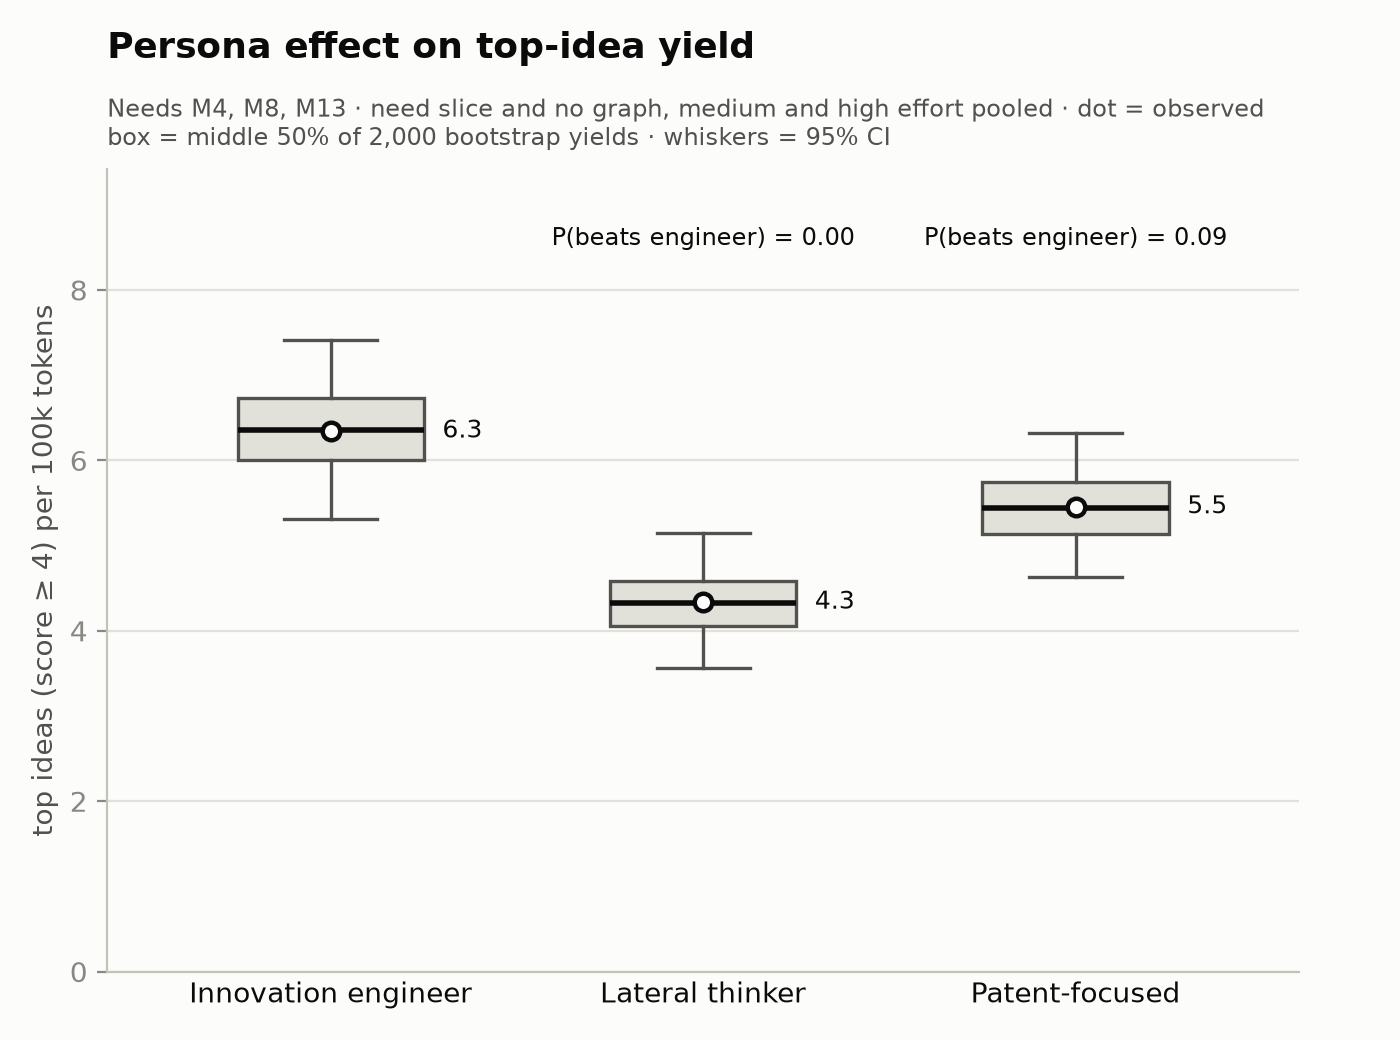
\includegraphics[width=0.7\textwidth]{figures/11_persona_effect.png}}{\fbox{\parbox[c][5cm][c]{0.9\textwidth}{\centering\small missing: \texttt{\detokenize{figures/11_persona_effect.png}}}}}
\caption{Persona follow-up: yield per persona over all of its calls (market-need slice and no graph, medium and high effort). Box = middle 50\% of 2,000 bootstrap yields, whiskers = 95\% CI, dot = observed.}
\label{fig:persona}
\end{figure}

\textbf{One yield per persona} (all its calls: both representations, both efforts; Figure \ref{fig:persona}, \texttt{11\_persona\_effect.png}):

\begin{longtable}[]{@{}
  >{\raggedright\arraybackslash}p{(\columnwidth - 6\tabcolsep) * \real{0.3276}}
  >{\raggedright\arraybackslash}p{(\columnwidth - 6\tabcolsep) * \real{0.2241}}
  >{\raggedright\arraybackslash}p{(\columnwidth - 6\tabcolsep) * \real{0.1724}}
  >{\raggedright\arraybackslash}p{(\columnwidth - 6\tabcolsep) * \real{0.2759}}@{}}
\toprule\noalign{}
\begin{minipage}[b]{\linewidth}\raggedright
Persona
\end{minipage} & \begin{minipage}[b]{\linewidth}\raggedright
Yield {[}95\% CI{]}
\end{minipage} & \begin{minipage}[b]{\linewidth}\raggedright
P(beats engineer)
\end{minipage} & \begin{minipage}[b]{\linewidth}\raggedright
Mean patentability {[}95\% CI{]}
\end{minipage} \\
\midrule\noalign{}
\endhead
\bottomrule\noalign{}
\endlastfoot
Innovation engineer & 6.3 {[}5.3--7.4{]} & -- & 2.19 {[}2.15--2.22{]} \\
Patent-focused & 5.5 {[}4.6--6.3{]} & 0.10 & 2.23 {[}2.19--2.27{]} \\
Lateral thinker & 4.3 {[}3.5--5.2{]} & \textless{} 0.001 & 2.17 {[}2.13--2.21{]} \\
\end{longtable}

P = share of 2,000 paired bootstrap draws (calls resampled within market need) in which the persona's yield is higher than the engineer's. The patent persona's yield is higher than the lateral thinker's in 97\% of draws.

\begin{itemize}
\tightlist
\item
  \textbf{No persona beat the plain engineer per token.} The engineer is the most efficient overall (the patent persona is behind but not clearly worse); the lateral thinker the least, most of all without a graph (5.8\% top ideas, against 9.3\% for the engineer). The new personas also cost slightly more per call: their descriptions add about 150 input tokens, and the patent persona thinks longer (about 11.7k output tokens per high-effort slice call, against 9.6k for the engineer).
\item
  \textbf{The slice helped every persona's top-idea rate,} and the lateral thinker most: its rate nearly doubles with the slice (5.8\% to 11.0\%). A persona that works by reframing seems to need concrete product structure to anchor on.
\item
  \textbf{The best single cell} is the patent persona with the slice at high effort: 18.0\% top ideas, and the only B ÷ C ratio whose interval clears 1 (1.55 {[}1.03--2.61{]}). It is one cell of twelve and is reported as a pattern.
\item
  \textbf{On these three market needs, the engineer's slice does not beat no graph} (B ÷ C 0.84 {[}0.60--1.22{]} pooled; at medium effort no graph is even ahead, 10.0 against 6.4, intervals overlapping). In the main study, too, no graph's yield at high effort (6.4) was close to the slice's (5.9); the slice's clear lead there came at medium effort on all 13 market needs (8.8), and on M4, one of the three market needs here, no graph did well. The slice's efficiency advantage over no graph is therefore market-need-dependent; its advantage over the full graph and the random slice is the robust result.
\item
  \textbf{The exemplars were not copied:} at most 1.8\% of ideas mention Wi-Fi, the Eurostar or entertainment (engineer baseline 0.7\%), and none mention Dyson, cyclones or bagless designs.
\end{itemize}

\textbf{Against the hypotheses written down before the run:}

\begin{itemize}
\tightlist
\item
  \textbf{H5 (the lateral thinker needs the graph less): not supported.} The B ÷ C ratio points the other way (1.16 against the engineer's 0.84), and the intervals overlap.
\item
  \textbf{H6 (the patent persona needs the graph more, for patentable ideas): not testable.} The judge rated almost every idea 2 out of 5 for patentability (means 2.13--2.31 in every cell); only about 1\% of ideas reach the pre-set threshold of 4, 0--2 per cell, so patentable yields are noise.
\item
  \textbf{H7 (personas do what they are told): not supported.} The lateral thinker's ideas are not rated more novel (mean novelty 3.23, against 3.30--3.34 for the engineer), and the patent persona's mean patentability is barely higher (2.23 {[}2.19--2.27{]} against 2.19 {[}2.15--2.22{]}; a difference of 0.04 on a 1--5 scale, intervals overlapping).
\end{itemize}

\textbf{Reading these results.} The quality rubric (relevance, novelty, feasibility, specificity) rewards concrete engineering, and the operator is SUBSTITUTE; a persona that proposes changes of perception rather than of parts may be marked down by the rubric rather than be worse. Patentability is the judge's estimate without a prior-art search; that it rates nearly all ideas as weakly patentable is consistent with many top ideas reusing known moves (solid-state RF, RF thawing), but it is not a legal assessment. Both are planned for the human check.

\hypertarget{change-from-the-pilot}{%
\subsection{Change from the pilot}\label{change-from-the-pilot}}

The pilot (2 market needs × 3 replicates) found the full graph winning 17 of 18 set comparisons. At full scale (13 market needs, 65 pairs) A's set-level advantage shrinks to about 64\%, and on the tail measure it disappears. The pilot's ``more novel but less feasible'' pattern for A did not replicate (it now describes no graph, C). The effort effect and the B-high vs A-low result held. Contrary to the pilot's expectation, quality kept rising from high to xhigh.

\hypertarget{caveats}{%
\subsection{Caveats}\label{caveats}}

\begin{itemize}
\tightlist
\item
  \textbf{Single judge model,} with no human calibration yet; a ``top idea'' is one the judge rates highly on relevance, novelty, feasibility and specificity together, a grounded strong idea rather than necessarily the wildest one.
\item
  \textbf{Coarse scores:} individual scores move in 0.25 steps, so the threshold (4.0, top 12.3\%) is the nearest available cut, and the 4.25 tail has too few ideas to separate arms.
\item
  \textbf{Yield assumes a constant rate per token.} The observed running counts are close to straight lines (Figure \ref{fig:yield}), but they depend on the order in which calls are taken; the slope itself does not.
\item
  \textbf{Budget curves assume independent calls} within a market need and use a small-sample estimate of each market need's success rate; they are a model, not observed sequences.
\item
  \textbf{R and C were run only at high effort;} R vs C was not judged pairwise, so whether a random slice beats no graph on whole sets is unknown.
\item
  \textbf{Relevance vs size rests on the tail measure:} the pairwise judging found no difference between B and R.
\item
  \textbf{R is size-matched to B in nodes, not tokens} (17\% fewer input tokens).
\item
  \textbf{Length and effort are intertwined;} the pairwise effort effects may be partly inflated by detail bias.
\item
  \textbf{xhigh covers 6 of 13 market needs,} which are slightly easier than average for top ideas; see the matched-needs results.
\item
  \textbf{One product, one operator, one prompt.} The worked example comes from the M8 branch of the graph, which may favour ideas in that area.
\item
  \textbf{Per-market-need results} rest on 5 calls or pairs each and should be read as patterns; the slice-size effect is exploratory (13 market needs, p ≈ 0.04--0.13).
\end{itemize}

\hypertarget{discussion-and-conclusion}{%
\section{Discussion and conclusion}\label{discussion-and-conclusion}}

\hypertarget{conclusions}{%
\subsection{Conclusions}\label{conclusions}}

This study asked how much of a product's knowledge graph an LLM needs to see in order to brainstorm well, measured not by the quality of its output alone but by how efficiently it turns tokens into good ideas. An innovation matrix \citep{Tchirsky} of a microwave oven (123 nodes, 246 edges) was given to \texttt{claude-haiku-5-5} in four forms: the full graph (A), the vertical slice for the target market need (B), a random slice of the same size (R), or no graph at all (C). The model applied the SUBSTITUTE operator to 13 market needs, with 5 replicates per cell and four levels of thinking effort. The 2,892 resulting ideas were judged blind by \texttt{claude-sonnet-5-5}, both as whole sets side by side and one idea at a time.

Brainstorming is a search for the rare great idea, so the main measure was the \textbf{yield}: top ideas (the top ∼12\% of all ideas) found per 100k tokens spent. Counted against tokens, top ideas accumulate in a straight line for every arm, so arms can be compared by slope. Five conclusions follow.

\begin{enumerate}
\def\labelenumi{\arabic{enumi}.}
\item
  \textbf{A relevant slice of the graph finds top ideas fastest.} The market-need slice at medium effort yields 8.8 top ideas per 100k tokens, about three times the full graph at any effort (2.6--3.2). The advantage over the full graph holds market need by market need: the slice is more efficient on 10 of 13 market needs (sign test p = 0.039), and its lead looks largest where the slice is small (exploratory).
\item
  \textbf{More context buys better average sets, not more great ideas.} Judged as whole sets, the full graph beats the slice (64\%) and no graph (74\%), mainly by being more specific. But its top-idea rate is no higher than the slice's, and its calls cost about twice as much, so per token it finds fewer top ideas than giving the model no graph at all (3.1 against 6.4 at high effort).
\item
  \textbf{Relevance matters, size does not.} A random slice of the same size as the market-need slice is the least efficient graph form: the market-need slice's slope is higher in 99\% of paired bootstrap draws (5.9 against 4.1 at high effort), and no graph beats the random slice on 10 of 12 market needs (p = 0.039). Irrelevant structure is worse per token than none. Judged as whole sets, market-need slice and random slice cannot be told apart: relevance shows up in the best ideas, not in the average set.
\item
  \textbf{Thinking effort raises quality, not efficiency.} High effort beats low in about 93\% of set comparisons, and extra-high effort gives the highest top-idea rates (19--21\%). But each call costs proportionally more, so yield does not rise with effort: the full graph stays at about 3 top ideas per 100k tokens from low to extra-high, and the slice peaks at medium effort.
\item
  \textbf{A persona prompt is no substitute for the right context (exploratory).} In a follow-up on three market needs, neither a lateral-thinker persona nor a patent-focused persona beat the plain innovation engineer per token (6.3 top ideas per 100k tokens against 5.5 and 4.3), and the hypotheses that they would change which representation works best were not supported. The lateral thinker was the least efficient, especially without a graph; given the market-need slice, its top-idea rate nearly doubled. The judge rated almost no idea from any persona as clearly patentable.
\end{enumerate}

Taken together: \textbf{to find great ideas efficiently, show the model the part of the product that bears on the problem, let it think moderately, and run it many times}, rather than giving it everything and asking it to think hard once. Which representation to use is a more durable decision than which model to use, because it keeps paying off as models change.

\textbf{Parsimony versus holism.} The results read as a contest between Ockham's razor and holistic thinking, with a twist. The razor says not to multiply entities \emph{beyond necessity}, and here the target market need defines what is necessary: the market-need slice, the graph cut to what the problem requires, is the most efficient form. Less context is not better as such: a random slice of the same size is the least efficient graph form, and no graph at all only matches the slice on some market needs. The full graph is the holistic bet, that distant parts of the product interact, and it does buy more specific ideas and better sets, but in calls aimed at one market need it pays for the whole product to reach the same market need from further away. Which principle wins depends on whether the problem has been framed \citep{Dorst2011}: \emph{once the problem is framed, parsimony beats holism per token; before it is framed, holism may be what finds the frame.} The open brainstorm proposed below tests the second half of that sentence.

\hypertarget{implications-for-design-thinkers-and-practitioners}{%
\subsection{Implications for design thinkers and practitioners}\label{implications-for-design-thinkers-and-practitioners}}

\begin{itemize}
\item
  \textbf{Frame before you generate.} The market-need slice is a machine version of a familiar design move: narrowing the problem to the functions, components and technologies that serve one user need before ideating. In this study that framing was worth more than exhaustive context, and more than asking the model to think harder. A well-built product graph lets a team cut that frame automatically, for any need.
\item
  \textbf{Budget LLM brainstorming by yield.} The useful question is not ``how good is the average idea?'' but ``how many great ideas does a given spend buy?'' Many cheap, focused calls beat a few expensive, all-knowing ones. A team can plan an ideation session like a test campaign: pick the representation with the best yield, set a budget, run the calls, filter the tail.
\item
  \textbf{Don't give the model everything just because you can.} Long contexts are easy to assemble and feel thorough. Here the full graph made top-idea generation about three times less efficient than the right slice, and an irrelevant slice was worse than nothing. What goes into the prompt should be chosen as deliberately as who is in the workshop.
\item
  \textbf{Don't expect a persona to do the work of the context.} Asking the model to think like a lateral thinker or a patent-minded inventor did not make it more efficient, and did not make its ideas more novel or more patentable in the judge's eyes. The representation of the problem mattered more than the role the model was asked to play.
\item
  \textbf{Curation becomes the human's main job.} Every arm produced strong and weak ideas side by side; even the best arm's top ideas are about one in seven. The value of the human shifts from generating ideas to recognising and developing the few good ones. Tools should make that triage fast: score, cluster, surface the tail.
\item
  \textbf{The product graph is a reusable, auditable design asset.} Building the innovation matrix once pays off across every market need, operator and session, and each idea anchors to named nodes and proposes new nodes and edges, so a team can see where in the product an idea intervenes and what it would change.
\item
  \textbf{Recurring themes are a signal.} The best ideas from many arms converged on the same moves (solid-state RF replacing the magnetron; low-frequency RF thawing). When independent runs keep arriving at one idea, it is a strong candidate for development, and the convergence itself is a cheap form of validation.
\end{itemize}

\hypertarget{new-research-directions}{%
\subsection{New research directions}\label{new-research-directions}}

\begin{itemize}
\item
  \textbf{Graph-guided search instead of single prompts.} Use the graph to steer a sequence of calls: pick a market need, slice, generate, score, then expand the slice around the anchors of the best ideas and generate again. Brainstorming becomes an explicit search over the product structure, with yield as its objective.
\item
  \textbf{Learning which slice to show.} The vertical slice was fixed by rule. Slices could instead be selected by retrieval or graph centrality, or learned from which nodes appear in top ideas. The slice-size pattern suggests that smaller, more focused slices may be more efficient still.
\item
  \textbf{Open brainstorming without a target market need.} Every call here targeted one market need, so the full graph's extra context could only reach for the same market need from further away. In an open brainstorm, where the model chooses where in the product to innovate, the full graph may play a role no slice can.
\item
  \textbf{Operators as graph transformations.} SUBSTITUTE, TRIZ principles and SCAMPER moves can each be defined as operations on the graph (replace a component node, merge two functions, remove a constraint edge), so ideas can be checked for whether they perform the operation they claim, and operators compared by the changes they produce.
\item
  \textbf{Ideas written back into the graph.} Accepted ideas could be merged into the graph, so the product model grows with every session and later runs build on earlier ones: a living design knowledge base.
\item
  \textbf{Yield as a standard measure.} Top ideas per token is simple, transferable and does not saturate. It could become a standard way to report LLM ideation, alongside or instead of mean scores that hide the differences that matter.
\end{itemize}

\hypertarget{what-should-be-tested-next}{%
\subsection{What should be tested next}\label{what-should-be-tested-next}}

In order of priority.

\begin{enumerate}
\def\labelenumi{\arabic{enumi}.}
\item
  \textbf{Human validation of the judge (planned).} Three raters with engineering or product background rate a blind, stratified sample of 99 ideas (\texttt{human\_check.py}), and the persona study's ideas are added to the sample. Report agreement between raters and with the judge, and above all whether ideas the judge places in the top tail are also rated highest by people. This also tests whether the quality rubric is unfair to perception-changing ideas such as the lateral thinker's.
\item
  \textbf{Extend the persona study.} Add the full graph as a third representation for each persona, and a persona-specific rubric (for example a perception-change criterion for the lateral thinker), to separate a weaker persona from a rubric that does not see what it is good at. Patentability needs a prior-art-aware judge: without one, the judge's ratings stayed near 2 of 5 for every persona.
\item
  \textbf{A second product and a second operator.} Repeat the core arms (B and C at medium effort, A at high effort) on a different product graph, ideally from another domain, and with at least one TRIZ principle and one more SCAMPER operator, to move the claim from ``one microwave, one operator'' towards a general result.
\item
  \textbf{Close the open comparisons.} Judge R against C on whole sets, and run R and C at medium effort, where the market-need slice was most efficient.
\item
  \textbf{Test the slice-size effect directly.} Vary the size of the slice for the same market need (for example by depth of the walk down the matrix) and measure yield, to confirm that smaller, more focused context is more efficient and to find where it stops helping.
\item
  \textbf{Replace the 5-ideas-per-call format.} Test 1, 5 and 10 ideas per call at equal total budget; if one idea per call yields more top ideas per token, the format itself has been holding the tail back.
\item
  \textbf{More replicates for the tail.} Twenty calls per market need for the leading arms would tighten the per-market-need estimates and allow the stricter top-idea threshold (≥ 4.25) to separate arms.
\item
  \textbf{Other judges and other generators.} Re-score a subset with a second judge model, and run the generation with a larger model, to test whether a stronger model needs less, or makes better use of more, context.
\item
  \textbf{Remove or swap the prompt's worked example.} The example came from the M8 branch of the graph; a run without it, or with an example from another branch, would show how much it steers the ideas.
\item
  \textbf{From ideas to outcomes.} Take the top ideas from each arm into an expert review or concept-development exercise, and record which ones practitioners would actually pursue: the final test of whether the judge's top tail is the one that matters in practice.
\end{enumerate}
